%
% Modelo de trabalho acadêmico (Teses, Dissertações, TCC)
% Documento principal
%
% Centro Federal de Educação Tecnológica de Minas Gerais - CEFET-MG
% Autor: Cristiano Fraga G. Nunes <cfgnunes@gmail.com>
%
% Projeto hospedado em: https://github.com/cfgnunes/latex-cefet-mg
%
%
% Informações:
%   Codificação utilizada: UTF-8
%   Tamanho da tabulação: 4 (espaços)


\documentclass[oneside]{abntex2-cefetmg}            % Imprimir apenas frente
%\documentclass[doubleside]{abntex2-cefetmg}        % Imprimir frente e verso

% Importações de pacotes
\usepackage[alf, abnt-emphasize=bf, bibjustif, recuo=0cm, abnt-etal-cite=2, abnt-etal-list=0]{abntex2cite}  % Citações padrão ABNT
\usepackage[utf8]{inputenc}                         % Acentuação direta
\usepackage[T1]{fontenc}                            % Codificação da fonte em 8 bits
\usepackage{graphicx}                               % Inserir figuras
\usepackage{amsfonts, amssymb, amsmath}             % Fonte e símbolos matemáticos
\usepackage{booktabs}                               % Comandos para tabelas
\usepackage{verbatim}                               % Texto é interpretado como escrito no documento
\usepackage{multirow, array}                        % Múltiplas linhas e colunas em tabelas
\usepackage{indentfirst}                            % Endenta o primeiro parágrafo de cada seção.
\usepackage{microtype}                              % Para melhorias de justificação?
\usepackage{palatino}                               % Usa a fonte Palatino
\usepackage[algoruled, portuguese]{algorithm2e}     % Escrever algoritmos
\usepackage{float}                                  % Utilizado para criação de floats
\usepackage[printonlyused,withpage]{acronym}
%\usepackage[bottom]{footmisc}                      % Mantém as notas de rodapé sempre na mesma posição
%\usepackage{times}                                 % Usa a fonte Times
%\usepackage{lmodern}                               % Usa a fonte Latin Modern
%\usepackage{subfig}                                % Posicionamento de figuras
%\usepackage{scalefnt}                              % Permite redimensionar tamanho da fonte
%\usepackage{color, colortbl}                       % Comandos de cores
%\usepackage{lscape}                                % Permite páginas em modo "paisagem"
%\usepackage{ae, aecompl}                           % Fontes de alta qualidade
%\usepackage{picinpar}                              % Dispor imagens em parágrafos
%\usepackage{latexsym}                              % Símbolos matemáticos
%\usepackage{upgreek}                               % Fonte letras gregas

% Inclui o preâmbulo do documento
%
% Documento: Preâmbulo
%

\titulo{Persistência Poliglota}
% \title{Polyglot Persistence}
% \subtitulo{Subtítulo do trabalho}
\autor{José Francisco Campos Limongi}
\local{Belo Horizonte}
\data{Agosto de 2014}
\instituicao{Centro Federal de Educação Tecnológica de Minas Gerais}
\programa{Curso de Engenharia de Computação}
\tipotrabalho{Monografia}
\preambulo{Modelo canônico de trabalho monográfico acadêmico em conformidade com as normas ABNT apresentado à comunidade de usuários \LaTeX.}
\orientador{Evandrino Barros}
%\orientador[Orientadora:]{Nome da orientadora}
\instOrientador{Centro Federal de Educação Tecnológica de Minas Gerais -- CEFET-MG}
% \coorientador{Nome do coorientador}
%\coorientador[Coorientadora:]{Nome da coorientadora}
% \instCoorientador{Centro Federal de Educação Tecnológica de Minas Gerais -- CEFET-MG}
%\areaconcentracao{Modelagem Matemática e Computacional}
%\linhapesquisa{Sistemas Inteligentes}


% Define as cores dos links e informações do PDF
\makeatletter
\hypersetup{
    portuguese,
    colorlinks,
    linkcolor=blue,
    citecolor=blue,
    filecolor=blue,
    urlcolor=blue,
    breaklinks=true,
    pdftitle={\@title},
    pdfauthor={\@author},
    pdfsubject={\imprimirpreambulo},
    pdfkeywords={abnt, latex, abntex, abntex2}
}
\makeatother

% Redefinição de labels
\renewcommand{\algorithmautorefname}{Algoritmo}
\def\equationautorefname~#1\null{Equa\c c\~ao~(#1)\null}

% Cria o índice remissivo
\makeindex

% Início do documento
\begin{document}

    % Retira espaço extra obsoleto entre as frases.
    \frenchspacing

    % Elementos pré textuais
    \pretextual
    %
% Documento: Capa
%

\makeatletter
\begin{capa}

    \hspace{-2.0cm}
    \begin{minipage}{0.19\textwidth}
        
\includegraphics[width=0.8\textwidth]{./04-figuras/cefet_logo}
    \end{minipage}
    \quad
    \hspace{-1.5cm}
    \begin{minipage}{.9\textwidth}
        \begin{center}
        \normalfont\scshape{\imprimirinstituicao}\\
        \normalfont\scshape{\imprimirprograma}\\
        \abntex@ifnotempty{\imprimirareaconcentracao}
        {%
            \normalfont\scshape{\imprimirareaconcentracao}
        }
        \end{center}
    \end{minipage}

    \vspace*{200pt}

    \begin{center}
        \ABNTEXchapterfont\Large\scshape\imprimirtitulo
        \abntex@ifnotempty{\imprimirsubtitulo}{%
            {\ABNTEXchapterfont\Large\scshape: }{\ABNTEXchapterfont\large\scshape\imprimirsubtitulo}
        }
    \end{center}

    \vspace*{80pt}

    \begin{center}
        \large\normalfont\scshape\textbf\imprimirautor
    \end{center}

    \vspace*{10pt}

    \begin{center}
        \small\imprimirorientadorRotulo{} \imprimirorientador \\
        \small\imprimirinstOrientador \\
        \abntex@ifnotempty{\imprimircoorientador}
        {%
            \begin{SingleSpacing}\par\end{SingleSpacing}
            \small\imprimircoorientadorRotulo{} \imprimircoorientador \\
            \small\imprimirinstCoorientador
        }
    \end{center}

    \vspace*{\fill}

    \begin{center}
        \normalfont\scshape{\imprimirlocal}\\
        \normalfont\scshape{\imprimirdata}
    \end{center}

\end{capa}
\makeatother
              % Capa
    %
% Documento: Folha de rosto
%

\makeatletter
\begin{folhaderosto}

    \begin{center}
        {\large\normalfont\scshape\textbf\imprimirautor}
    \end{center}

    \vspace*{150pt}

    \begin{center}
        \ABNTEXchapterfont\Large\scshape\imprimirtitulo
        \abntex@ifnotempty{\imprimirsubtitulo}{%
            {\ABNTEXchapterfont\Large\scshape: }{\ABNTEXchapterfont\large\scshape\imprimirsubtitulo}
        }
    \end{center}

    \vspace*{90pt}

  

    \vspace*{\fill}

    \begin{center}
        \normalfont\scshape{\imprimirinstituicao}\\
        \normalfont\scshape{\imprimirprograma}\\
        \normalfont\scshape{\imprimirlocal}\\
        \normalfont\scshape{\imprimirdata}
    \end{center}

\end{folhaderosto}
\makeatother
        % Folha de rosto
    %
% Documento: Folha de aprovação
%

\makeatletter
\begin{folhadeaprovacao}

    \begin{center}
        {\large\normalfont\scshape\textbf\imprimirautor}
    \end{center}

    \vspace*{50pt}

    \begin{center}
        \ABNTEXchapterfont\Large\scshape\imprimirtitulo
        \abntex@ifnotempty{\imprimirsubtitulo}{%
            {\ABNTEXchapterfont\Large\scshape: }{\ABNTEXchapterfont\large\scshape\imprimirsubtitulo}
        }
    \end{center}

    \vspace*{60pt}

    \abntex@ifnotempty{\imprimirpreambulo}{%
        \SingleSpacing
        \begin{tabular}{p{.24\textwidth}p{.15\textwidth}p{.44\textwidth}}
            & \multicolumn{2}{p{.6\textwidth}}{\small\hyphenpenalty=10000{\imprimirpreambulo}} \\ & & \\
        \end{tabular}
    }

    \vspace*{10pt}

    \begin{center}
        Trabalho aprovado. \imprimirlocal, 22 de janeiro de 2015
    \end{center}

    \begin{center}
        \assinatura{\textbf{\imprimirorientador} \\ Orientador}
        \assinatura{\textbf{Professor} \\ Anolan Yamilé Milanés Barrientos}
        \assinatura{\textbf{Professor} \\ Bruno André Santos}
        %\assinatura{\textbf{Professor} \\ Convidado 3}
        %\assinatura{\textbf{Professor} \\ Convidado 4}
    \end{center}

    \vspace*{\fill}

    \begin{center}
        \normalfont\scshape{\imprimirinstituicao}\\
        \normalfont\scshape{\imprimirprograma}\\
        \normalfont\scshape{\imprimirlocal}\\
        \normalfont\scshape{\imprimirdata}
    \end{center}

\end{folhadeaprovacao}
\makeatother
    % Folha de aprovação
    %%
% Documento: Dedicatória
%

\begin{dedicatoria}

Espaço reservado para dedicatória.
Inserir seu texto aqui...

\end{dedicatoria}
       % Dedicatória
    %%
% Documento: Agradecimentos
%

\begin{agradecimentos}

Inserir seu texto aqui...
(esta página é opcional)

\end{agradecimentos}
    % Agradecimentos
    %
% Documento: Epígrafe
%

\begin{epigrafe}

\textit{``Seja realista, exija o impossível.'' (Roland Castro)}

\end{epigrafe}
          % Epígrafe
    % %
% Documento: Resumo (Português)
%

\begin{resumo}

Persistência poliglota é a utilização de mais de um banco de dados para uma mesma aplicação. Em um sistema podemos ter algum conjunto de dados que deve ter alta disponibilidade, e outro conjunto de dados que deve ser consistente. Devido a essa diferença de necessidades surgiu a persistência poliglota. Utilizando-a podemos armazenar em um banco, que garante disponibilidade, o conjunto de dados que precisa de alta disponibilidade e podemos armazenar em outro banco, que favorece a consistência, o conjunto de dados que precisa ser consistente. Visando esse problema, criamos duas aplicações semelhantes ao Twitter, sendo uma com a persistência monoglota, que utiliza apenas o banco de dados MongoDB e a outra com persistência poliglota que utiliza o banco de dados MongoDB e Redis. Fizemos a comparação entre esses dois sistemas sobre duas funcionalidades, a leitura da \textit{feed} de \textit{tweets} e a inserção de um \textit{tweet}. Com o modelo criado utilizando persistência poliglota, conseguimos melhorar o tempo de leitura da \textit{feed} de \textit{tweets}, porém o tempo de inserção do \textit{tweet} piorou. Percebemos que a persistência poliglota possibilitou uma melhora no desempenho em parte da aplicação. Por isso, podemos afirmar que o modelo escolhido não foi ideal para ressaltar as vantagens de um sistema que utiliza persistência poliglota, mas demonstramos que a utilização da persistência poliglota pode melhorar muito o desempenho da aplicação.


\textbf{Palavras-chave}: Banco de dados. Persistência poliglota. NoSQL. Desempenho. 

\end{resumo}          % Resumo na língua vernácula
    % %
% Documento: Resumo (Inglês)
%

\begin{resumo}[Abstract]


Polyglot persistence is a system that use more than one database. In a system can have a set of data that must be available, and another set of data that must be consistent. The need to maintain these two types of data, did rise the polyglot persistence. Thus, the set of data, that needs to be available are stored in a database, that favors availability, and the set of data, that needs to be consistent are stored in a database, that favors consistency.We created two applications similar to Twitter, one using just MongoDB database, and another using Redis and MongoDB databases. We did tests to compare the spent in reading the tweet feed and the time spent to insert a tweet. With the polyglot persistence the time spent in reading the feed of tweets was lower and the time spent to insert was higher. Therefore, the model choosen was not the ideal for the Twitter similar system, but we proved that polyglot persistence can improve the performance of the application.

\textbf{Keywords}: Database. Polyglot Persistence. NoSQL. Performance. 

\end{resumo}
          % Resumo em língua estrangeira
    %
% Documento: Lista de figuras
%

\pdfbookmark[0]{\listfigurename}{lof}
\listoffigures*
\cleardoublepage
      % Lista de figuras
    %
% Documento: Lista de tabelas
%

\pdfbookmark[0]{\listtablename}{lot}
\listoftables*
\cleardoublepage
      % Lista de tabelas
    %%
% Documento: Lista de quadros
%

\pdfbookmark[0]{\listofquadrosname}{loq}
\listofquadros*
\cleardoublepage
      % Lista de quadros
    %%
% Documento: Lista de algoritmos
%

\newcommand{\algoritmoname}{Algoritmo}
\renewcommand{\listalgorithmcfname}{Lista de Algoritmos}

\floatname{algocf}{\algoritmoname}
\newlistof{listofalgoritmos}{loa}{\listalgoritmoname}
\newlistentry{algocf}{loa}{0}

\counterwithout{algocf}{chapter}
\renewcommand{\cftalgocfname}{\algoritmoname\space}
\renewcommand*{\cftalgocfaftersnum}{\hfill--\hfill}

\pdfbookmark[0]{\listalgorithmcfname}{loa}
\listofalgorithms
\cleardoublepage
   % Lista de algoritmos
    %
% Documento: Lista de abreviaturas e siglas
%

\pdfbookmark[0]{\listofsiglasname}{lot}
\listofsiglas*
\begin{acronym}
  \acro{SQL}{Structured Query Language}
  \acro{Redis}{Remote Dictionary Server}
  \acro{SGBD}{Sistema de Gerenciamento do Banco de Dados}
  \acro{UML}{Unified Model Language}
  \acro{UoD}{Universo de Discurso}
  \acro{ACID}{Atomicidade, Consistência, Isolamento e Durabilidade}
  \acro{XML}{\textit{eXtensible Markup Language}}
  \acro{MVC}{\textit{Model View Controller}}
\end{acronym}

\cleardoublepage       % Lista de abreviaturas e siglas
    % %
% Documento: Lista de símbolos
%

\begin{simbolos}
    \item[$ \Gamma $] Letra grega Gama
    \item[$ \lambda $] Comprimento de ondada
    \item[$ \in $] Pertence
\end{simbolos}
     % Lista de símbolos
    %
% Documento: Sumário
%

\pdfbookmark[0]{\contentsname}{toc}
\tableofcontents*
\cleardoublepage           % Sumário

    % Elementos textuais
    \textual
    \chapter{Introdução}\label{chap:introducao}
A necessidade de persistência de dados sempre esteve presente na computação. A medida que os sistemas evoluíram a complexidade da forma que os dados eram armazenados aumentou significativamente. Com isso, houve a necessidade da criação de um sistema computadorizado de manutenção de registros \cite{CJDate}, o banco de dados.

O modelo relacional foi um dos primeiros modelos que surgiram, sua estrutura são tabelas de duas dimensões com linhas e colunas. Os dados armazenados são tipados, podendo variar a quantidade de tipos de acordo com o banco utilizado. Para interagir com esse modelo é necessário realizar consultas com a linguagem \ac{SQL}. Alguns exemplos de banco de dados relacional são MySQL\footnote{Sítio oficial  \url{http://www.mysql.com}}, Oracle\footnote{Sítio oficial  \url{http://www.oracle.com/technetwork/oem/db-mgmt/db-mgmt-093445.html}} e PostgreSQL\footnote{Sítio oficial \url{http://www.postgresql.org/}}.

Durante anos, o banco de dados relacional tem sido considerado a melhor opção para os problemas de escalabilidade, porém surgiram novas soluções com novas alternativas de estruturas de dados, replicação simples, alta disponibilidade e novos métodos de consultas \cite{SDSW}. Essas opções são conhecidas como NoSQL ou banco de dados do modelo não-relacional

Existem diversos gêneros de banco de dados do modelo não-relacional, entre eles chave-valor, orientado a documento, orientado a coluna e orientado a nó. Com o surgimento dessas novas soluções, o questionamento sobre qual banco de dados é melhor para resolver certo tipo de problema, vem à tona. A partir disso, o conhecimento e compreensão sobre os bancos de dados em geral se torna necessário para realizar uma boa escolha.

Entendendo que cada banco se destaca em determinados tipos de problema, é nítido perceber que sistemas que trabalham com mais de um banco de dados podem oferecer um melhor desempenho, dando origem à persistência poliglota.

Este trabalho consiste na comparação de dois sistemas baseados em NoSQL. O primeiro utilizará apenas um banco de dados, que será do gênero orientado a documento. O segundo utilizará dois bancos de dados, sendo um do gênero orientado a documento e um outro banco do gênero chave-valor. O segundo sistema, por utilizar dois bancos de dados, caracteriza a persistência poliglota, que é alvo desse trabalho. Os bancos escolhidos para fazer esses sistemas foram o MongoDB e o \ac{Redis}. O autor escolheu esses bancos de dados por ter experiência na linguagem \textit{Ruby on Rails}, que oferece excelentes bibliotecas para esses bancos e por serem utilizados em diversas aplicações. O MongoDB está sendo utilizado em grandes empresas, como Cisco, eBay, Codeacademy, Microsoft, Craiglist, The Guardian e outras, conforme sítio oficial do MongoDB\footnote{\url{http://www.mongodb.com/customers}}. O \ac{Redis} está sendo utilizado no Twitter, Github, Craiglist e outros conforme referência do sítio oficial\footnote{\url{http://redis.io/topics/whos-using-redis}}.
O intuito desse trabalho é comparar desempenho do uso da persistência poliglota  com a persistência monoglota.

MongoDB é um banco de dados do gênero orientado a documento e foi desenhado para trabalhar com grande volume de dados. O próprio nome é uma derivação da palavra inglesa \textit{humongous} que significa gigantesco. O diferencial desse banco é a maneira com que os registros são armazenados. Cada registro fica armazenado em um documento que é análogo à tupla do modelo relacional. O documento é composto por um identificador único e um conjunto de valores de tipos e estruturas aninhadas. Esse banco é bem flexível, pois não tem esquema pré-definido e permite valores multivalorados. Ao criarmos a arquitetura do sistema, temos que identificar se as entidades criadas são expressivas como um documento \cite{SDSW}. Além disso, há soluções para tratar concorrência e foi desenhado para trabalhar em ambientes distribuídos. A linguagem utilizada para fazer consulta no MongoDB é JavaScript. Nesse trabalho utilizaremos o banco MongoDB nos dois sistemas que serão criados.

O segundo banco utilizado se chama \ac{Redis} que é do gênero chave-valor. Esse tipo de armazenamento é mais simples. Como o próprio nome indica, é armazenado um valor para determinada chave. O valor armazenado pode ter uma estrutura variável. Escolhemos esse banco, pois, antes de efetivar as operações em disco, ele mantém os dados na memória primária. Dessa forma, o banco tem um ganho muito alto em desempenho, porém poderá ocorrer perda de dados, caso ocorra uma falha de hardware \cite{SDSW}. A forma de estruturar esse banco é muito parecida com o tipo estruturado de dados chamado \textit{hash}, que é implementado em algumas linguagens de computação, como Java e Ruby. Esse banco será utilizado no segundo sistema a ser desenvolvido.


\section{Motivação}
\label{sec:motivacao}
A persistência poliglota é uma alternativa para melhorar o desempenho de uma aplicação. Utilizando-a, conseguimos adaptar cada tipo de problema a um gênero de banco de dados.

Exitem duas variáveis opostas no ambiente da persistência de dados: consistência e disponibilidade. Quanto mais consistente um dado, menos disponível ele será e quanto mais disponível um dado menos, consistente ele estará \cite{NoSQL}. Em aplicações é comum termos um conjunto de dados que deve ser sempre consistente e um outro conjunto de dados que deve estar sempre disponível. Por exemplo, em um sistema de \textit{e-commerce} é necessário que os dados do carrinho de compra estejam sempre disponíveis e os dados dos produtos em estoque devem estar consistentes. Após confirmado a compra dos produtos do carrinho de compra, temos que verificar a consistência desses dados, ou seja, verificar se há esses produtos no estoque. Dessa forma, os usuários têm uma boa experiência ao selecionar o produto e quando efetivarem a compra, a loja não terá problemas com estoque.

Logo, podemos utilizar dois gêneros de banco de dados para atender a esses conjuntos. Um que garante disponibilidade e outro que garante  consistência. Utilizando esse ambiente misto, é esperado que haja um ganho de desempenho.

Atualmente poucos trabalhos apresentam uma comparação entre sistemas que utilizam apenas um gênero de banco (persistência monoglota)  e sistemas que utilizam persistência poliglota. 

Com esse trabalho pretendemos ilustrar as diferenças entre a persistência monoglota e poliglota, destacando as vantagens que a persistência poliglota pode oferecer. Fizemos a implementação de dois sistemas similares ao Twitter\footnote{Twitter é uma rede social, na qual usuários podem fazer publicações em texto de até cento e quarenta caracteres. Cada usuário possui um perfil e pode acompanhar as publicações de outros usuários. Para fazer esse acompanhamento, basta começar a seguir o usuário desejado.}, porém um utiliza a persistência monoglota e outro utiliza a persistência poliglota. Coletamos resultados de duas partes do sistema: leitura do \textit{feed} de \textit{tweets} e inserção de um \textit{tweet}. Esses resultados indicaram que a persistência poliglota aumentou significativamente o desempenho na leitura do \textit{feed}, mas devido ao modelo utilizado, piorou o sistema na inserção de um \textit{tweet}.

O trabalho está organizado em cinco capítulos, o próximo, \autoref{chap:fundamentacaoTeorica}, apresenta a fundamentação teórica necessária para fazer esse trabalho. O \autoref{chap:implementacao} explica os sistemas criados e a diferença de implementação entre eles. O \autoref{chap:resultados} apresenta os resultados preliminares que demonstraram um melhor desempenho da persistência poliglota e, por fim, o \autoref{chap:conclusao} apresenta a conclusão do trabalho.





            % Introdução
    % %
% Documento: Trabalhos Relacionados
%

\chapter{Trabalhos Relacionados}

Este capítulo inclui muitas citações bibliográficas. Os principais
itens de bibliografia citados são livros, artigos em conferências,
artigos em {\textit journals} e páginas Web. A bibliografia deve seguir o
padrão ABNT\index{ABNT}\footnote{Este não é o endereço oficial da
ABNT pois as Normas Técnicas oficiais são pagas e não estão disponíveis na Web.}.

A bibliografia é feita no padrão {\ttfamily bibtex}.
As referências são colocadas em um arquivo separado.
Os elementos de cada item bibliográfico que devem constar na bibliografia são apresentados a seguir.

Para livros, o formato da bibliografia no arquivo fonte é o seguinte:

\begin{verbatim}
@Book{linked,
   author = {A. L. Barabasi},
   title = {Linked: The New Science of Networks},
   publisher = {Perseus Publishing},
   year = {2002},
}
\end{verbatim}

A citação deste livro se faz da seguinte forma \verb#\cite{linked}# e o resultado fica assim \cite{linked}.
Para os artigos em {\textit journals}, veja por exemplo \cite{acmsurveys},
descrito da seguinte forma no arquivo {\ttfamily .bib}:

\begin{verbatim}
@article{acmsurveys,
   author    = {Deepayan Chakrabarti and Christos Faloutsos},
   title     = {Graph mining: Laws, generators},
   journal   = {ACM Computing Surveys},
   volume    = {38},
   number    = {1},
   year      = {2006},
   pages     = {2-59},
   publisher = {ACM},
   address   = {New York, NY, USA},
}
\end{verbatim}

O artigo \cite{3faloutsos} foi publicado em conferência. Embora
às vezes seja difícil distinguir um artigo publicado em {\textit
 journal} de um artigo publicado em conferência, esta distinção é
fundamental. Em caso de dúvida, procure ajuda de seu orientador.

Veja também duas citações juntas \cite{rp99,mar00} e como citar
endereços Web \cite{irl:06}.
O trabalho realizado para editar as citações no formato correto é
compensado por uma bibliografia impecável.

\section{Citações livres}\label{citacoesLivres}
Citações são trechos transcritos ou informações retiradas das publicações consultadas para a realização do trabalho.
As citações são utilizadas no texto com o propósito de esclarecer, completar, embasar ou corroborar as ideias do autor.

Todas as publicações consultadas e efetivamente utilizadas (através de citações) devem ser listadas, obrigatoriamente, nas referências bibliográficas, de forma a preservar os direitos autorais e intelectuais.

Na utilização de citações, normalmente, utiliza-se referências.
Para cada tipo de referência presente no texto será apresentado um exemplo do comando utilizado para criá-lo.

Há basicamente dois tipos de citações: citações livres e citações literais.

Nas citações livres, reproduzem-se as ideias e informações de um autor, sem, entretanto, ``copiar letra por letra'' o texto do autor.
Há várias maneiras de se fazer uma citação livre, como mostra os exemplos abaixo.

Por outro lado, \citeonline{maturana:2003} defende um princípio de lógica.
Para o autor, quando dizemos \ldots

Além disso, \citeonline{teste:2004} argumenta que \ldots\mbox{ }Observe o detalhe do termo \textit{et al}.
que deve ser utilizado quando o trabalho citado possui mais de três autores.
Esse recurso é automatizado pelo estilo {\ttfamily abntex2}\index{ABNT!abntex2}.
Caso não haja desejo em abreviar o nome dos demais autores através do termo \textit{et al.}, deve-se incluir a opção {\ttfamily abnt-no-etal-label}.

Para evitar uma interrupção na sequência do texto, o que poderia, eventualmente, prejudicar a leitura, pode-se indicar a fonte entre parênteses imediatamente após a citação livre.
Porém, neste caso específico, o nome do autor deve vir em caixa alta, seguido do ano da publicação, como no exemplo a seguir.

A física, então, constituiu-se como a prova mínima da efetividade do método científico para descobrir as verdades do universo \cite{teste:2004,maturana:2003}.


\section{Citações literais}\label{citacoesLiterais}
Nas citações literais, reproduzem-se as ideias e informações de um autor, exatamente como este a expressou, ou seja, faz-se uma ``cópia letra por letra'' do texto do autor.
Há várias maneiras de se fazer uma citação literal, como mostra os exemplos abaixo.

As citações longas (mais de 3 linhas) devem usar um parágrafo específico para ela, na forma de um texto recuado (4 cm da margem esquerda), com tamanho de letra menor do aquela utilizada no texto e espaçamento simples entre as linhas, seguido dos sobrenomes dos autores em caixa alta (separados por ponto e vírgula), ano de publicação e número da página.
Veja o exemplo abaixo.

\begin{citacao}
Desse modo, opera-se uma ruptura decisiva entre a reflexividade filosófica, isto é a possibilidade do sujeito de pensar e de refletir, e a objetividade científica.
Encontramo-nos num ponto em que o conhecimento científico está sem consciência.
Sem consciência moral, sem consciência reflexiva e também subjetiva.
Cada vez mais o desenvolvimento extraordinário do conhecimento científico vai tornar menos praticável a própria possibilidade de reflexão do sujeito sobre a sua pesquisa \cite[p.~28]{morinmoigne:2000}.
\end{citacao}

Para se criar o efeito demonstrado na citação anterior, deve-se utilizar o comando:
\begin{verbatim}
    \begin{citacao}
        <citacao>
    \end{citacao}
\end{verbatim}

Opcionalmente, pode-se referenciar os autores no corpo de texto (neste caso seus nomes devem vir em minúsculas), e em seguida colocar a citação literal, em um novo parágrafo recuado.
Note que pode após a citação literal não mais aparece o nome dos autores, visto que já se encontra no texto.
Veja o exemplo seguinte.

\citeonline[p.~33]{morinmoigne:2000}, ao fazerem as suas críticas à ciência, explicitam uma ideia coletiva:

\begin{citacao}
Mas o curioso é que o conhecimento científico que descobriu os meios realmente extraordinários para, por exemplo, ver aquilo que se passa no nosso sol, para tentar conceber a estrutura das estrelas extremamente distantes, e até mesmo para tentar pesar o universo, o que é algo de extrema utilidade, o conhecimento científico que multiplicou seus meios de observação e de concepção do universo, dos objetos, está completamente cego, se quiser considerar-se apenas a si próprio!
\end{citacao}

As citações curtas (menos de 3 linhas) devem ser inseridas diretamente no texto (entre aspas), seguida do nome do autor (em caixa alta), ano e página, como no exemplo a seguir.

Então significa apenas que ``assumo que não posso fazer referência a entidades independentes de mim para construir meu explicar'' \cite[p.~35]{maturana:2003}.

O conhecimento de \citeonline[p.~35]{maturana:2003} aponta que isto significa apenas que ``assumo que não posso fazer referência a entidades independentes de mim para construir meu explicar''.

Finalmente, e isto vale para citações curtas ou longas, caso seja necessário inserir, no meio de uma citação uma palavra ou frase curta de sua autoria, que sirva para clarear ou completar a frase do autor citado, isto deve ser feito colocando a citação entre aspas.
O comentário deverá ser inserido sem aspas.
Ou seja, todo texto da citação deverá ficar envolvido por aspas.
O exemplo abaixo apresenta o resultado esperado.

Significa apenas que ``assumo que não posso fazer referência a entidades'' objetivas no sentido tradicional ``independentes de mim para construir meu explicar'' {\citeonline[p.~35]{maturana:2003}}.

\section{Informações sobre as referências utilizadas}\label{referenciasUtilizadas}

Nesta seção serão apresentadas os comandos necessários para a criação das referências utilizadas anteriormente.
As informações serão apresentadas da seguinte maneira:

\begin{itemize}
    \item \citeonline{maturana:2003}\\ \verb|\citeonline{maturana:2003}|
    \item \citeonline{teste:2004}\\ \verb|\citeonline{teste:2004}|
    \item \cite[p.~28]{morinmoigne:2000}\\ \verb|\cite[p.~28]{morinmoigne:2000}|
    \item \citeonline[p.~33]{morinmoigne:2000}\\ \verb|\citeonline[p.~33]{morinmoigne:2000}|
    \item \cite[p.~35]{maturana:2003}\\ \verb|\cite[p.~35]{maturana:2003}|
    \item \citeonline[p.~35]{maturana:2003}\\ \verb|\citeonline[p.~35]{maturana:2003}|
    \item \cite{teste:2004,maturana:2003}\\ \verb|\cite{teste:2004,maturana:2003}|
\end{itemize}
 % Trabalhos relacionados
    \chapter{Fundamentação Teórica}
\label{chap:fundamentacaoTeorica}


Para entendermos o porquê de utilizar mais de um banco de dados em uma mesma aplicação, temos que entender o que é um banco de dados, quais gêneros existem e para qual tipo de problema cada gênero se destaca.

Este capítulo está organizado em duas seções, a \autoref{sec:database} apresenta o conceito de banco de dados e a \autoref{sec:databasetype} apresenta os gêneros de bancos de dados mais utilizados atualmente. A \autoref{sec:databasetype} se divide em três subseções, a \autoref{subsec:relationaldatabasetype} apresenta o conceito do modelo relacional, a \autoref{subsec:nosqldatabasetype} apresenta o conceito do modelo não-relacional comparada com o conceito do modelo relacional e a \autoref{subsec:polyglotpersitence} apresenta o conceito de persistência poliglota.

\section{Banco de Dados}
\label{sec:database}

Banco de dados é um sistema computadorizado de manutenção de registros, análogo à um armário de arquivamento eletrônico. Podemos entendê-lo como um repositório para manter a coleção de arquivos de dados computadorizados \cite{CJDate}. \citeonline{Elmasri} define banco de dados como uma coleção de dados relacionados e que dados são fatos com um significado implícito. Porém, a definição de \citeonline{Elmasri} é mais abrangente, logo ele aponta três propriedades implícitas para restringir a definição de banco de dados.

A primeira propriedade é que um banco de dados deve representar alguns aspectos do mundo real, chamado de \textit{\ac{UoD}}. As alterações que ocorrem nesse universo são refletidas em um banco de dados. A segunda propriedade define que o banco de dados é uma coleção lógica e coerente de dados com algum significado inerente, ou seja, uma coleção de dados randômicos não pode ser considerado um banco de dados. A terceira propriedade afirma que banco de dados é projetado, construído e povoado com dados, atendendo a uma proposta específica. Além disso, possui um grupo de usuários definido e algumas aplicações preconcebidas, de acordo com o interesse desse grupo.

Os bancos de dados têm contribuído para o aumento do uso do computador \cite{Elmasri} e podemos afirmar que eles apresentam um papel crucial em quase todas as áreas em que os computadores são utilizados. Devido a essa importância o estudo sobre banco de dados é extremamente necessário para os profissionais da computação.

Antes da existência dos bancos de dados, a aplicação devia gerenciar e processar arquivos para manter os dados persistidos. Para justificar o uso de banco de dados, \citeonline{Elmasri} cita quatro características: natureza autodescritiva, abstração de dados, suporte para as múltiplas visões de dados e processamento de transações de multiusuários.

A primeira característica, natureza autodescritiva do banco de dados, apresenta o catálogo do banco de dados como uma grande vantagem sobre o processamento tradicional dos arquivos, pois o catálogo identifica as estruturas dos arquivos, formato e tipo de dados. Logo, não é necessário conhecer a aplicação para trabalhar com os dados. Já  o processamento tradicional dos arquivos, mantém essas definições de estrutura na própria aplicação \cite{Elmasri}.

Em relação à característica abstração de dados, \citeonline{Elmasri} afirma que não é feita no processamento tradicional de arquivos, pois é a aplicação que define a estrutura dos dados. Por exemplo, suponha que tenhamos diversos programas utilizando o mesmo arquivo para armazenar uma coleção de dados. Se um desses programas precisar de acrescentar algum campo novo, todos os outros programas que acessam esse arquivo, devem ser modificados para contemplar o novo campo adicionado. Já quando utilizamos banco de dados, a alteração da estrutura dos dados pode não influenciar no funcionamento dos outros programas.

Em relação à característica suporte para múltiplas visões dos dados, \citeonline{Elmasri} diz que quando é utilizado o banco de dados, é possível ter diferentes visões sobre os dados, fazendo o cruzamento das tabelas. Com a abordagem de processamento de arquivo tradicional, isso não é usual.

A última característica citada por \citeonline{Elmasri} é o processamento de transações multiusuários, essa característica é essencial para que várias aplicações possam acessar e alterar os dados a partir de usuários diferentes e simultâneos. Porém, o \ac{SGBD} deve ter implementado um controle de concorrência para garantir a atomicidade das transações e a consistência dos mesmos.

\citeonline{Elmasri} não cita a existência dos bancos de dados NoSQL, que são bancos que não têm esquema pré-definido, chamados de \textit{schemaless}. Apesar de não ter a declaração do tipo de estruturas de dados contidas no banco, os bancos de dados \textit{schemaless} fazem a abstração dos dados da mesma maneira que os bancos de dados tradicionais, têm suporte para múltipla visões e multiusuários.

Como revelado acima, a utilização do banco de dados facilita o desenvolvimento das aplicações, permite a abstração entre aplicação e dados e, além disso, faz o controle de concorrência. Após verificarmos que o uso de banco de dados é imprescindível, nos deparamos com uma outra dificuldade, qual banco de dados utilizar. Os bancos de dados, chamados de NoSQL, chamam a atenção da comunidade científica, depois da publicação de dois artigos BigTable \cite{bigtable} e Dynamo \cite{dynamo}. Essas publicações apresentam bancos de dados NoSQL que têm um desempenho superior ao modelo relacional. O BigTable apresenta um banco de dados orientado a coluna e o Dynamo apresenta um banco de dados chave-valor.

\section{Gêneros de Banco de dados}
\label{sec:databasetype}
Durante anos, o banco de dados relacional tem sido considerado a melhor opção para a maioria dos problemas de pequeno ou grande volume de dados. No entanto, o aumento do volume de dados fez com que os especialistas buscassem novas soluções, que permitissem o armazenamento paralelo dos dados, pois o modelo relacional não foi desenhado para funcionar em \textit{clusters}. Logo, os bancos de dados NoSQL se destacaram por funcionarem bem nesse ambiente e terem um melhor desempenho com grande volume de dados \cite{NoSQL}.

Os bancos de dados NoSQL têm as seguintes características: não usam o modelo relacional, foram desenhados para funcionar em \textit{clusters}, são \textit{open source} e não tem catálogos (\textit{schemaless}) \cite{NoSQL}. Carlo Strozzi foi o primeiro a utilizar o nome NoSQL, mas não no sentido que a palavra tem hoje. Strozzi denominou um banco de dados relacional, \textit{open source} de NoSQL, pois não usava \ac{SQL} como linguagem de consulta. O sentido, que a palavra tem hoje, veio de uma conferência realizada em São Francisco nos Estados Unidos, em Junho de 2009. Johan Oskarsson que organizou essa conferência, escolheu esse nome, porque era uma boa \textit{hashtag} no Twitter, pois era pequeno, memorável e tinha poucos resultados no Google. Isso facilitaria os interessados a encontrar a conferência. Apesar do termo não significar explicitamente o que são esses bancos de dados, atendeu bem a intenção de Oskarsson \cite{NoSQL}.


\subsection{Banco de dados Relacional}
\label{subsec:relationaldatabasetype}
O modelo relacional armazena os dados em tabelas de duas dimensões em linhas e colunas. A interação com esse banco é feito por um \ac{SGBD} que utiliza a \ac{SQL} como linguagem de consulta de dados. Os dados armazenados são valores tipados e podem ser numéricos, texto, data e outros tipos, que são configurados e forçados pelo sistema. É possível fazer junção das tabelas e obter diferentes perspectivas das informações de maneira simples. MySQL, Oracle e PostgreSQL são alguns exemplos de banco de dados relacional \cite{SDSW}.
A representação do modelo relacional pode ser feita com o diagrama \ac{UML}. Por exemplo, um sistema de \textit{e-commerce} poderia ser desenhado conforme o diagrama da \autoref{fig:diagrama_sql_uml} e as tuplas ficariam dispostas conforme \autoref{fig:disposicao_tabela}.
\begin{figure}[H]
    \centering
    \caption{Exemplo de um diagrama \ac{UML} para o modelo relacional}
    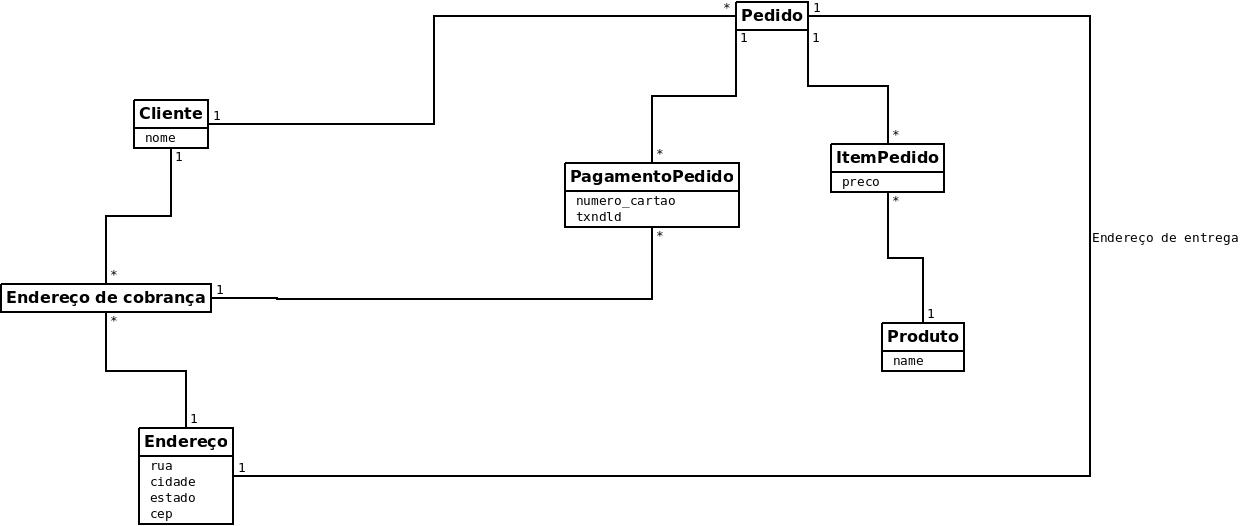
\includegraphics[width=0.8\textwidth]{./04-figuras/diagrama_sql_uml.jpg}
    \fonte{\cite{NoSQL}}
    \label{fig:diagrama_sql_uml}
\end{figure}
\begin{figure}[H]
    \centering
    \caption{Exemplo da disposição dos dados no modelo relacional}
    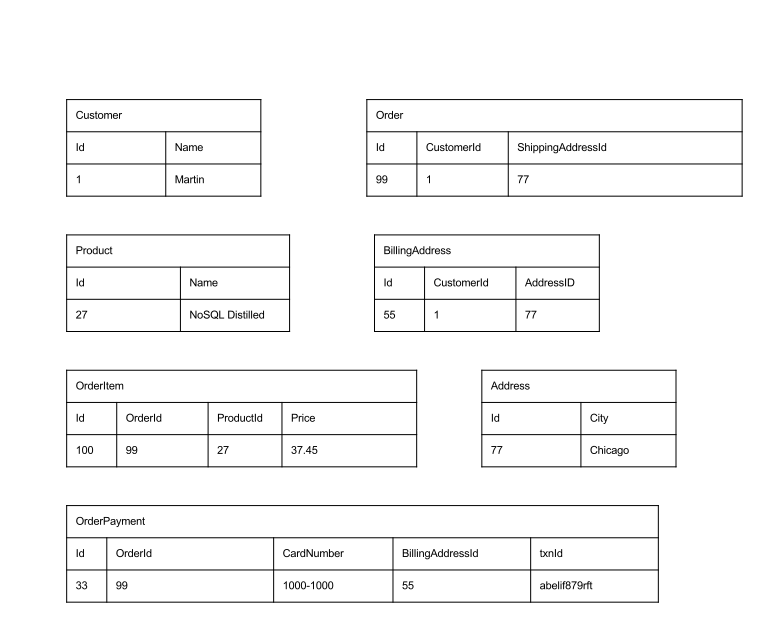
\includegraphics[width=0.8\textwidth]{./04-figuras/disposicao_dados_tabela.png}
    \fonte{\cite{NoSQL}}
    \label{fig:disposicao_tabela}
\end{figure}


O modelo relacional funciona muito bem para diversas aplicações, pois é bem flexível em relação às consultas, permite concorrência, transações e pode ser integrado com várias aplicações. Porém, há uma desvantagem que causa frustação em muitos desenvolvedores, chamada de Impedância de Correspondência ou \textit{Impedance Mismatch} \cite{Elmasri,NoSQL}. Isso ocorre, pois nem sempre o tipo do campo no banco de dados irá corresponder com o tipo esperado da linguagem utilizada, então é necessário criar uma forma de associação entre o tipo da variável da linguagem com o tipo do valor da tabela. Outra desvantagem é que esse não aceita valores multivalorados, distanciando a aplicação ainda mais do modelo relacional.


\subsection{Banco de dados não-relacional}
\label{subsec:nosqldatabasetype}
Os bancos de dados NoSQL foram construídos para suprir a necessidade de se trabalhar com grande quantidade de dados e em \textit{clusters}. NoSQL abrange diversos gêneros de banco de dados, entre eles o orientado a documento, chave-valor, orientado a coluna e orientado a nó.

Todos esses gêneros não possuem catálogo, ou seja, não se define previamente em qual estrutura os dados serão armazenados. Isso permite uma flexibilidade no sistema, pois a estrutura dos dados pode ser alterada facilmente. É possível adicionar um novo campo, sem ter que se preocupar com a atualização da base legada, pois os objetos de uma mesma coleção podem ter diferentes campos. Da mesma maneira, para remover um campo, basta parar de armazená-lo. Os registros antigos, que tinham esse campo, continuarão com eles e os objetos novos não irão armazenar esse campo, que já não faz parte da aplicação \cite{NoSQL}.

Com isso é possível trabalhar com dados não uniformes, isto é, dados que para cada registro há um conjunto diferente de atributos. Para que o banco de dados relacional lide com um objeto dessa natureza, é necessário uma tabela com os campos de todos os objetos e consequentemente, isso traria uma quantidade grande de campos vazios.

Basicamente, os bancos de dados NoSQL deslocam a definição do esquema para a aplicação que acessa o banco. Isso pode se tornar problemático quando há muitas aplicações acessando o mesmo banco, mas existem soluções para resolver isso. Uma delas seria encapsular toda a interação com o banco de dados, fazendo esse funcionar como um \textit{web service} \cite{NoSQL}.

Além dessa flexibilidade, a maioria dos gêneros NoSQL permite estruturar dados multivalorados \footnote{O banco de dados orientado a nó, é um dos gêneros que não implementam agregação.}. Esses dados são modelados como agregação, que é uma coleção de objetos relacionados que desejamos tratar como um único objeto \cite{domain-driven}. A agregação facilita a manipulação e a consistência desses dados, pois é tratado como uma unidade, ou seja, é lido e escrito sempre todo o conjunto de dados. Como, geralmente, ao utilizar esse relacionamento buscamos, operações atômicas, essa abordagem se adapta perfeitamente com a aplicação \cite{NoSQL}. Para exemplificar, iremos modelar o exemplo de
\textit{e-commerce} anterior de duas maneiras diferentes.

A primeira iremos utilizar agregação entre as relações de \textit{Pedido-Endereço}, \textit{Pedido-ItemPedido}, \textit{Pedido-Pagamento}, \textit{Cliente-Endereço}, e por fim \textit{Endereço-Pagamento}. No diagrama iremos utilizar o símbolo de composição em \ac{UML} para demonstrar como a informação se adapta na estrutura de agregação \cite{NoSQL}.O diagrama ficaria como a \autoref{fig:diagrama_no_sql_uml_simples} e a disposição de dados ficaria como a \autoref{fig:disposicao_json_simples}. É usual a utilização de JSON \footnote{JSON é um tipo de estrutura de dados muito utilizado em JavaScript que representa os dados estruturados de uma maneira simples para as pessoas lerem e escreverem e para as máquinas fazerem a conversão.} para mostrar os dados em NoSQL \cite{NoSQL}.

\begin{figure}[H]
    \centering
    \caption{Exemplo de um diagrama \ac{UML} utilizando agregação}
    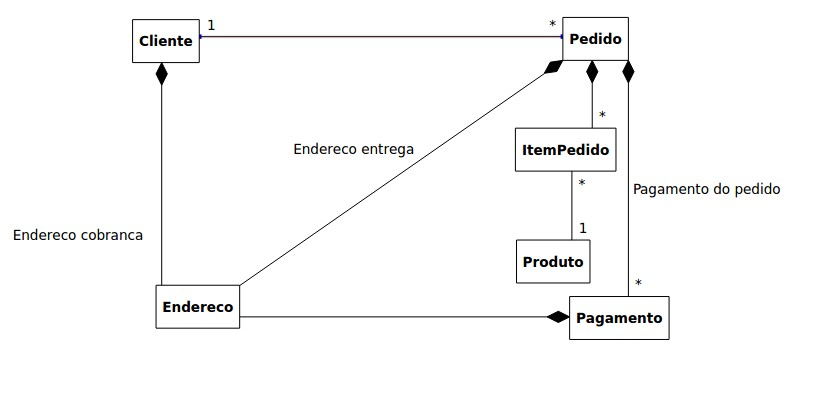
\includegraphics[width=0.8\textwidth]{./04-figuras/diagrama_no_sql_uml_simples.jpg}
    \fonte{\cite{NoSQL}}
    \label{fig:diagrama_no_sql_uml_simples}
\end{figure}
\begin{figure}[H]
    \centering
    \caption{Exemplo da disposição dos dados utilizando agregação}
    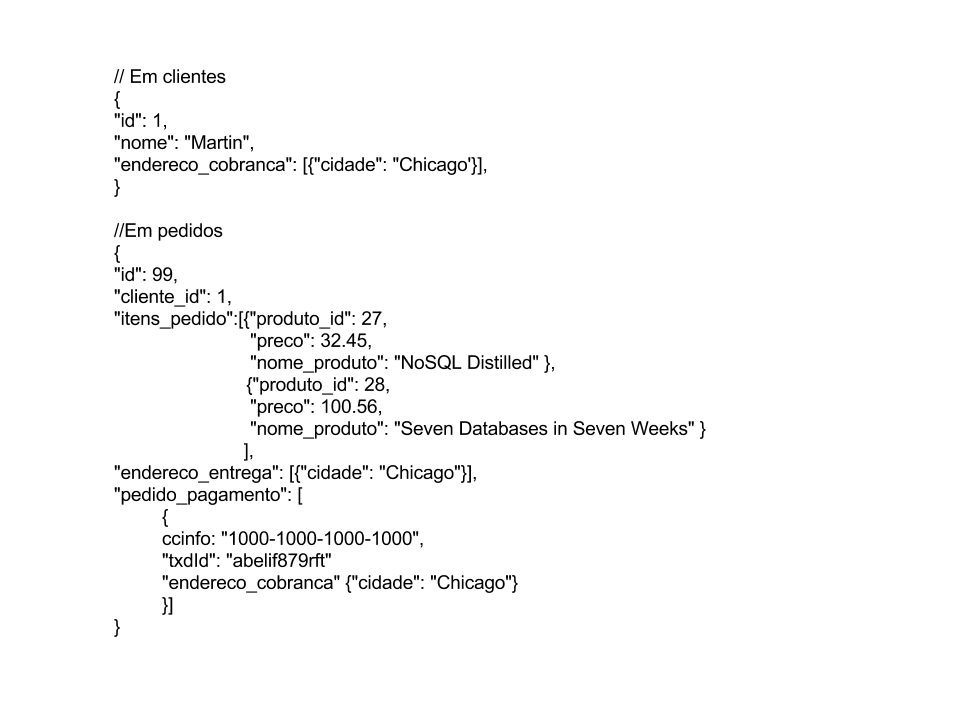
\includegraphics[width=0.8\textwidth]{./04-figuras/disposicao_json_simples.png}
    \fonte{\cite{NoSQL}}
    \label{fig:disposicao_json_simples}
\end{figure}



Observamos que as duas principais agregações são cliente e pedido. O cliente contém apenas uma lista, que é a de endereços. Já o pedido contém uma lista de itens de pedido, endereços e pagamentos. E por fim, o pagamento contém uma lista de endereços. Endereço aparece três vezes, mas ao invés de utilizar uma referência com um identificador, como no modelo relacional, o valor é copiado. Essa replicação de dados se adapta ao problema, pois, nesse caso, não queremos que o endereço em pagamento seja alterado caso o usuário altere o endereço de entrega.  Utilizando o modelo relacional temos duas maneiras de lidar com o problema. A primeira é tratar para que não seja permitido alterar o endereço, após desse ser vinculado à pedido ou pagamento. A segunda e mais usada, seria duplicar o endereço e associar à pedido ou à pagamento, ou seja, os dados são replicados da mesma maneira. As relações entre \textit{Pedido-Cliente} e \textit{ItemPedido-Produto} funcionam da mesma maneira que o modelo relacional, um lado da relação armazena o identificador do outro lado, por exemplo, o pedido mantém o identificador do cliente relacionado.

A segunda maneira de modelar o exemplo de \textit{e-commerce} em NoSQL, seria utilizar as agregações do exemplo anterior (\textit{Pedido-Endereço}, \textit{Pedido-ItemPedido}, \textit{Pedido-Pagamento}, \textit{Cliente-Endereço}, e por fim \textit{Endereço-Pagamento}) mais a agregação entre cliente e pedido. O modelo em \ac{UML} ficaria como a \autoref{fig:diagrama_no_sql_uml_duplo} e os dados ficariam dispostos como a \autoref{fig:disposicao_json_duplo}.

\begin{figure}[H]
    \centering
    \caption{Exemplo de um diagrama \ac{UML} para utilizando agregação entre cliente e pedido}
    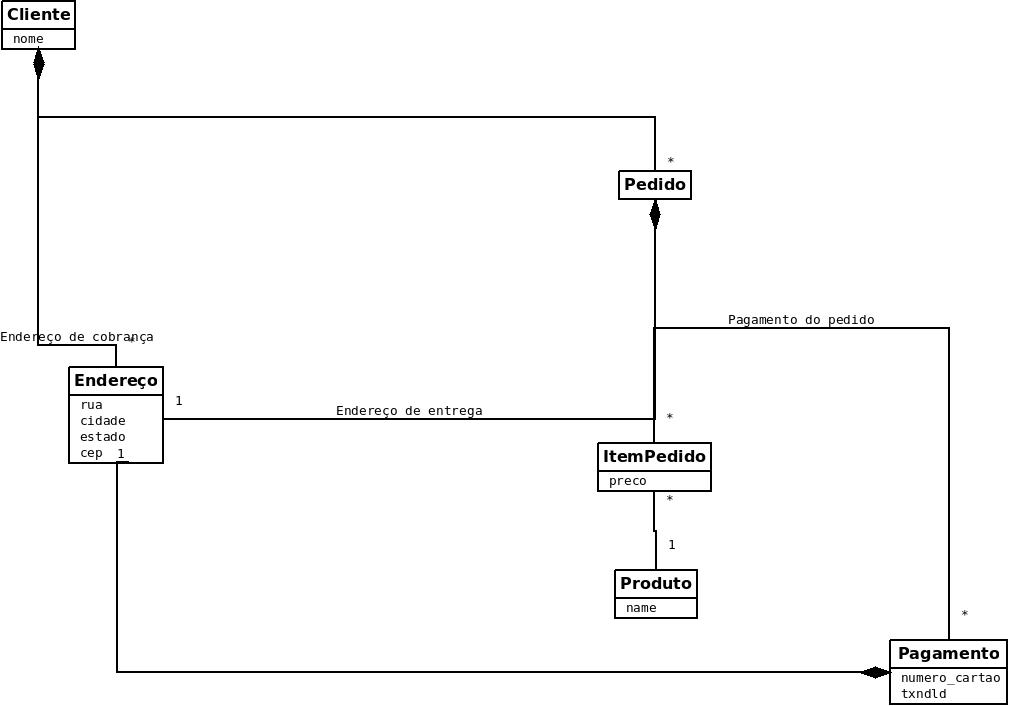
\includegraphics[width=0.8\textwidth]{./04-figuras/diagrama_no_sql_uml_duplo.jpg}
    \fonte{\cite{NoSQL}}
    \label{fig:diagrama_no_sql_uml_duplo}
\end{figure}
\begin{figure}[H]
    \centering
    \caption{Exemplo da disposição dos dados no NoSQL, utilizando agregação entre cliente e pedido}
    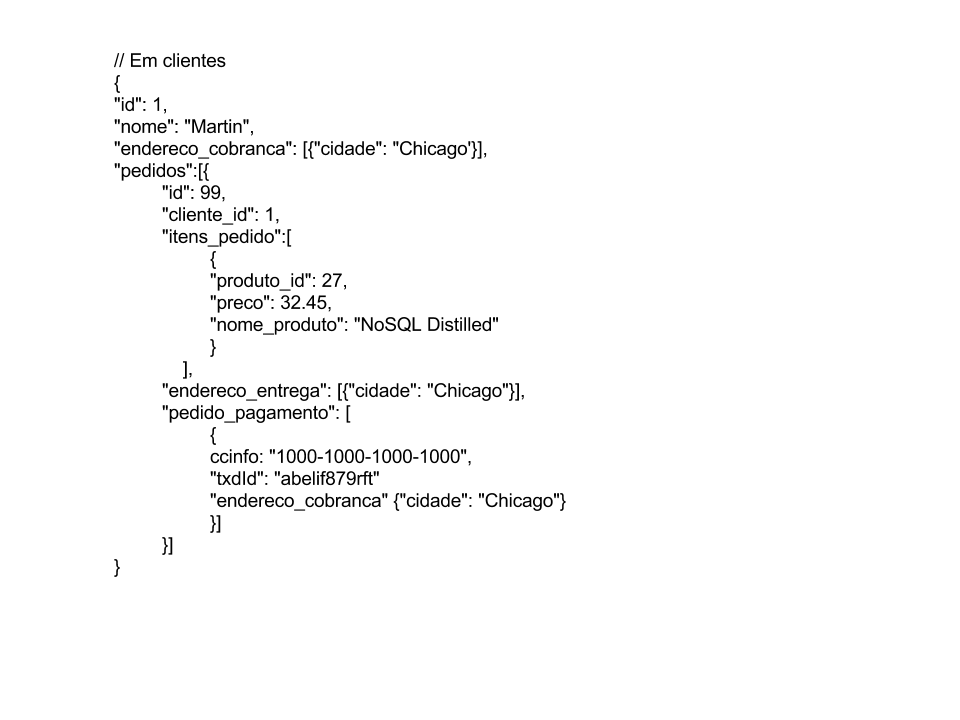
\includegraphics[width=0.8\textwidth]{./04-figuras/disposicao_json_duplo.png}
    \fonte{\cite{NoSQL}}
    \label{fig:disposicao_json_duplo}
\end{figure}

Como na maioria dos problemas de modelagem não existe a melhor solução, mas sim uma que se adapta melhor para um certo tipo de problema, devemos analisar o objetivo da aplicação para fazer uma melhor escolha.

Nesse exemplo se for interessante para a aplicação listar o histórico dos pedidos do mês corrente, o modelo da \autoref{fig:diagrama_no_sql_uml_duplo} não é o ideal, pois será necessário entrar em cada cliente para ler os pedidos. Já utilizando o modelo da \autoref{fig:diagrama_no_sql_uml_simples}, essa consulta do histórico se torna trivial \cite{NoSQL}, basta fazer uma busca dos pedidos que contém a data igual a do mês corrente.

Por outro lado, ao buscarmos os pedidos de um cliente, o modelo da \autoref{fig:diagrama_no_sql_uml_duplo} irá apresentar um melhor desempenho. Pois, será necessário apenas buscar o cliente que essa consulta irá trazer todos os pedidos. Já o modelo da \autoref{fig:diagrama_no_sql_uml_simples} será necessário percorrer pedido por pedido e comparar o identificador do cliente.

Outra razão para utilizar agregação é a facilidade proporcionada para colocar o funcionamento em \textit{clusters}. Pois, utilizando esse modelo temos a informação de quais dados devem ser manipulados juntos e se devem estar no mesmo nó do \textit{cluster}.

O modelo relacional por não tratar o conceito de agregação é chamado de \textit{aggregate-ignorant}. Apesar disso, o modelo relacional tem suas vantagens por não tratar. A principal é que ao utilizar o modelo relacional, podemos analisar os dados em diversas perspectivas, já no banco de dados NoSQL algumas consultas podem não ser complexas ou até mesmo mais lentas. Por exemplo, o modelo da \autoref{fig:diagrama_no_sql_uml_duplo} ficará mais lento para buscar o histórico de pedidos.

Outra desvantagem do NoSQL, é não implementar transações do tipo \ac{ACID}. Esses gêneros de banco de dados conseguem implementar essas transações apenas sobre uma agregação como dito anteriormente. Caso seja necessário o controle dessas transações, deverá ser feito no código da aplicação.

\subsection{Persistência Poliglota}
\label{subsec:polyglotpersitence}

O objeto desse trabalho são duas aplicações que utilizam dois gêneros de banco de dados, orientado a documento e chave-valor.

O gênero chave-valor funciona como uma simples tabela \textit{hash} que dado uma chave única encontrará um valor. O sistema desse banco não tem conhecimento algum sobre esse valor, logo poderá ser um texto, um objeto multivalorado, um valor binário. Qualquer tipo de informação, apenas o tamanho é limitado, dependendo do banco. Alguns exemplos de bancos desse gênero são \ac{Redis}\footnote{Sítio oficial do Redis \url{http://redis.io/}} e Riak\footnote{Sítio oficial do Riak \url{http://basho.com/riak/}}.
A consistência utilizando esse gênero existe apenas para operação realizada com uma chave. Então não temos consistência para um grupo de chaves. Isso pode ser implementado, mas é muito custoso \cite{NoSQL}. Em relação à consistência no ambiente paralelo, cada banco implementa de uma maneira. O Riak, por exemplo, utiliza o chamado \textit{Quorums}, que é uma abordagem de consistência que elege o valor mais atual fazendo uma consulta entre os nós. Aquele valor que tiver na maioria dos nós será eleito como mais atualizado.

Como o banco não tem conhecimento da estrutura armazenada, qualquer filtro necessário deverá ser feito pela aplicação. A aplicação faz a busca no banco utilizando a chave, o banco retorna o valor referente a essa chave e em seguida, a aplicação trabalha com esse valor fazendo o filtro dos registros que deseja. Também é possível programar o tempo de expiração da chave. Essa maneira que o banco chave-valor trabalha faz com que ele se adeque bem para manter dados da sessão de um usuário, carrinhos de compra de um \textit{e-commerce}, perfil de usuários e outros. Não é indicado para armazenar estruturas que a aplicação fará buscas comparando os dados do valor. Por exemplo, suponha que tenhamos o modelo da \autoref{fig:diagrama_no_sql_uml_duplo} para armazenar a estrutura utilizando o modelo chave-valor. Para realizar a busca de todos os pedidos do mês corrente, teremos que carregar para a aplicação todos os clientes, acessar os pedidos de cada um e verificar se a data do pedido é igual ao do mês corrente \cite{NoSQL}.

O gênero orientado a documento trabalha com o conceito de documento. Documento pode ser um \ac{XML}, JSON, BSON ou outros formatos. Esses documentos são armazenados em coleções. Documentos da mesma coleção são semelhantes, mas não precisam ser idênticos. Se fizermos uma analogia, a coleção seria a tabela no modelo relacional e um documento seria uma tupla no modelo relacional. Exemplos desse gênero são MongoDB \footnote{Sítio oficial do MongoDB \url{http://www.mongodb.com/}} e CouchDB \footnote{Sítio oficial do CouchDB \url{http://couchdb.apache.org/}}\cite{NoSQL}.
Existem dois tipos de relacionamento, um que funciona semelhante ao modelo relacional que é referenciando um documento de uma coleção pelo identificador, análogo a chave estrangeira no modelo relacional . Outro tipo é embutir documentos dentro de um documento, ou seja, agregação. Consistência existe apenas para os objetos da agregação, como relatado anteriormente. Quando distribuído, o MongoDB pode trabalhar com uma série de políticas de como irá se comportar no ambiente paralelo, que são configuráveis. Esse gênero não implementa transações\footnote{Operações de inserir, atualizar ou deletar com a opção de emitir o \textit{commit} ou \textit{rollback}}. O MongoDB permite que seja feito consultas com filtros e a linguagem utilizada é o JavaScript. Consultas mais complexas que utilizam os documentos embutidos em outros documentos são realizadas com \textit{MapReduce} \cite{NoSQL}. Por exemplo, se modelarmos esse banco com a o modelo da \autoref{fig:diagrama_no_sql_uml_duplo} para fazer a busca dos pedidos do mês corrente, diferente do \ac{Redis}, o banco é capaz de fazer esse filtro e retornar apenas os pedidos que têm a data igual a do mês corrente. Para isso ele utiliza \textit{MapReduce}.

Diferentes bancos de dados foram desenhados para resolver diferentes problemas \cite{NoSQL}. Conseguir identificar diferentes problemas de armazenamento, representação ou escalabilidade dentro de uma aplicação pode ser um indicativo que mais de um banco de dados deve ser utilizado. Da mesma maneira que diferentes paradigmas de linguagem de programação são utilizados em um desenvolvimento Web, diferentes gêneros de banco de dados podem ser usados em uma mesma aplicação \cite{multiparadigma}. É considerado persistência poliglota quando uma aplicação utiliza mais de um banco de dados.


  % Fundamentação teórica
    % %
% Documento: Metodologia
%

\chapter{Metodologia}

Este trabalho será realizado em três etapas.

A primeira etapa consiste do estudo dos bancos de dados escolhidos, buscando entender melhor como os dados são estruturados. Ainda nessa etapa, será feito uma pesquisa bibliográfica sobre sistemas que utilizam persistência poliglota. Essa pesquisa será fundamental para a próxima etapa, pois irá direcionar a criação da aplicação para que ressalte as diferenças de um sistema com persistência poliglota.

A segunda etapa consiste da criação de duas aplicações semelhantes ao Twitter, porém uma utilizará apenas um banco de dados e a outra utilizará dois bancos de dados. Essa aplicação terá as funcionalidades básicas do Twitter.

A terceira e última etapa é a comparação da performance das operações sobre os dados dessas aplicações. Logo, consiste na medição de tempo gasto para inserção, leitura, atualização e exclusão dos dados.

Para a realização desse trabalho será necessário de um computador com os servidores dos bancos de dados instalados.

\section{Implementação}
\label{sec:implementation}
Explicar a aplicação, como foi feito e apresentar os casos de uso

\section{Implementação Monoglota}
\label{sec:monoglot}
Apresentar os diagrama de classe da parte persistida e da aplicação como um todo, falar do framework MongoId, explicar a forma com que a associcao dos models

\section{Implementação Poliglota}
\label{sec:polyglot}
Apresentar os diagrama de classe da parte persistida e da aplicação como um todo, falar do framework do Redis, explicar onde foi usado um banco e onde foi usado outro.

\section{Coleta de dados}
\label{sec:data}
Explicar como foi coletado os dados
           % Metodologia
    \chapter{Implementação}
\label{chap:implementacao}

Para comparar os sistemas que utilizam apenas um banco de dados (persistência monoglota) com os sistemas que utilizam mais de um banco de dados (persistência poliglota) implementamos e testamos o desempenho desses.

Escolhemos fazer uma aplicação semelhante ao Twitter. Nessa aplicação, o usuário poderá se cadastrar, escrever \textit{tweets}, seguir outros usuários e listar os \textit{tweets} dos usuários que ele segue.

Este capítulo é dividido em duas seções, a primeira, \autoref{sec:useCase} descreve os casos de uso da aplicação. A \autoref{sec:applications} descreve os detalhes da implementação com persistência monoglota e com persistência poliglota.

\section{Casos de Uso}
\label{sec:useCase}
Essa seção irá descrever os casos de uso da aplicação. Cinco subseções foram criadas para detalhar os cinco casos de uso criados. A primeira \autoref{subsec:useCaseCreateUser}, detalha o caso de uso que descreve a funcionalidade de cadastro do usuário. A \autoref{subsec:useCaseCreateTweet} descreve o caso de uso de cadastro de um \textit{tweet}. A \autoref{subsec:useCaseUserFollow} apresenta o caso de uso que descreve como o usuário segue outro usuário. A \autoref{subsec:useCaseUserUnfollow} apresenta o caso de uso que descreve como o usuário para de seguir outro e por fim, a \autoref{subsec:useCaseFeed} descreve o último caso de uso que detalha como o usuário visualiza a \textit{feed}, página que apresenta todos os \textit{tweets} dos usuários que o usuário logado segue.


\subsection{Caso de Uso 1 - Cadastro do usuário}
\label{subsec:useCaseCreateUser}

Sumário: Usuário usa o sistema para se cadastrar

Ator primário: Usuário

Ator secundário: Sistema

Precondições: O usuário deverá ter uma email


Fluxo Principal\begin{enumerate}
{\setlength\itemindent{25pt}
    \item O usuário acessa o sistema;
    \item O sistema exibe a tela de entrada, \autoref{fig:telaInicial};
    \item O usuário clica em \textit{Sign up};
    \item O sistema retorna a tela com o formulário de cadastro de usuário, \autoref{fig:signup};
    \item O usuário preenche os campos de nome, email, senha e confirmação de senha;
    \item O sistema cria o usuário e redireciona para tela de \textit{My Tweets}, \autoref{fig:myTweets}.
}
\end{enumerate}

Fluxo de Exceção (5): Email inválido
\begin{enumerate}
{\setlength\itemindent{25pt}
\item Se o usuário não digitou um email válido, o sistema reporta o campo incorreto e retorna ao passo 5.
}
\end{enumerate}

Fluxo de Exceção (5): Campos obrigatórios não preenchidos
\begin{enumerate}
{\setlength\itemindent{25pt}
\item Se o usuário não preencher todos os campos, o sistema informa que os campos são obrigatórios e o usuário retorna ao passo 5.
}
\end{enumerate}

Fluxo de Exceção (5): Senha e confirmação de senha não conferem
\begin{enumerate}
{\setlength\itemindent{25pt}
\item Se o usuário não preencher as senhas corretamente, o sistema retorna ao passo 5, informando que as senhas não conferem.
}
\end{enumerate}

\begin{figure}[H]
    \centering
    \caption{Tela Inicial}
    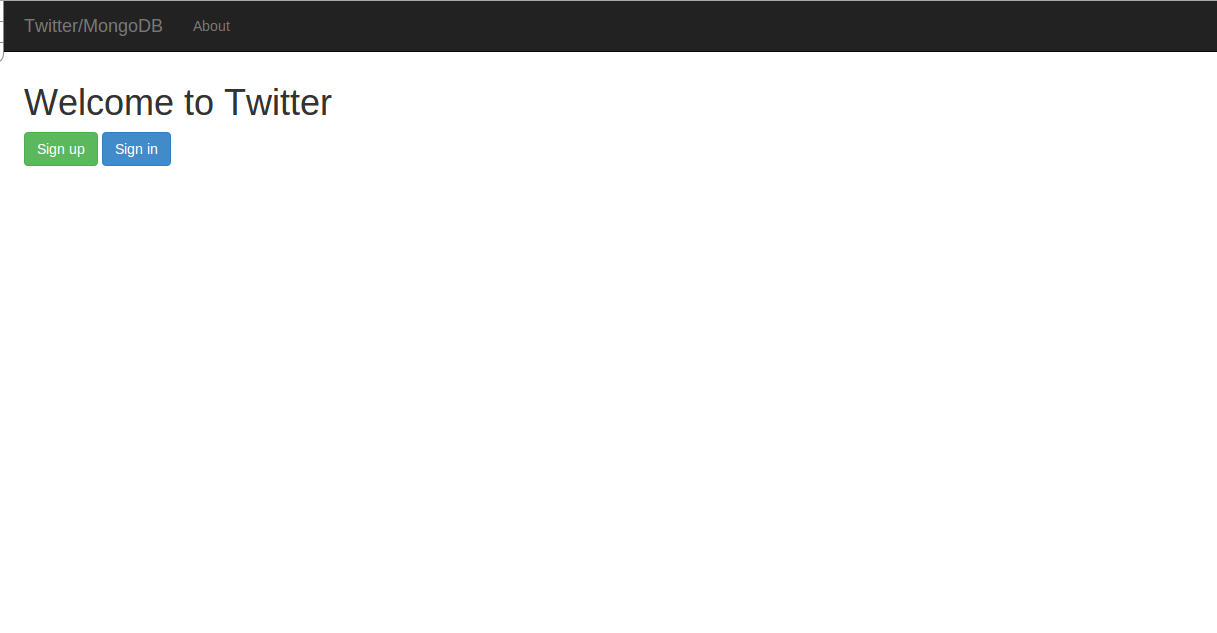
\includegraphics[width=0.8\textwidth]{./04-figuras/PrimeiraTela.png}
    \fonte{Autoria própria}
    \label{fig:telaInicial}
\end{figure}

\begin{figure}[H]
    \centering
    \caption{Tela de cadastro de usuário}
    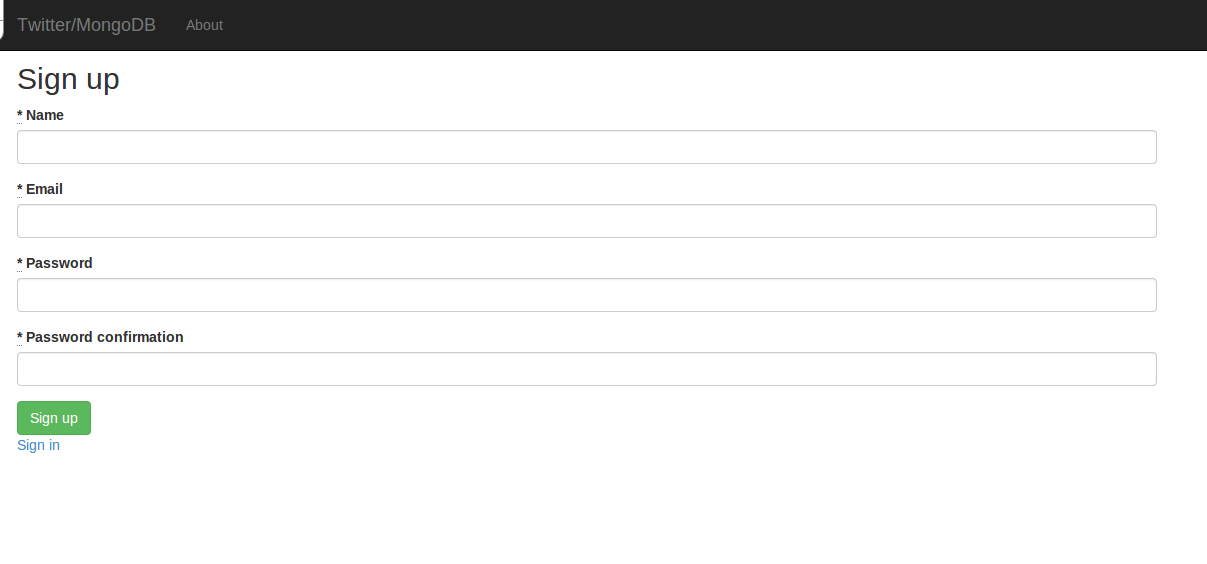
\includegraphics[width=0.8\textwidth]{./04-figuras/Signup.png}
    \fonte{Autoria Própria}
    \label{fig:signup}
\end{figure}

\begin{figure}[H]
    \centering
    \caption{Tela Tweets do Usuário Logado}
    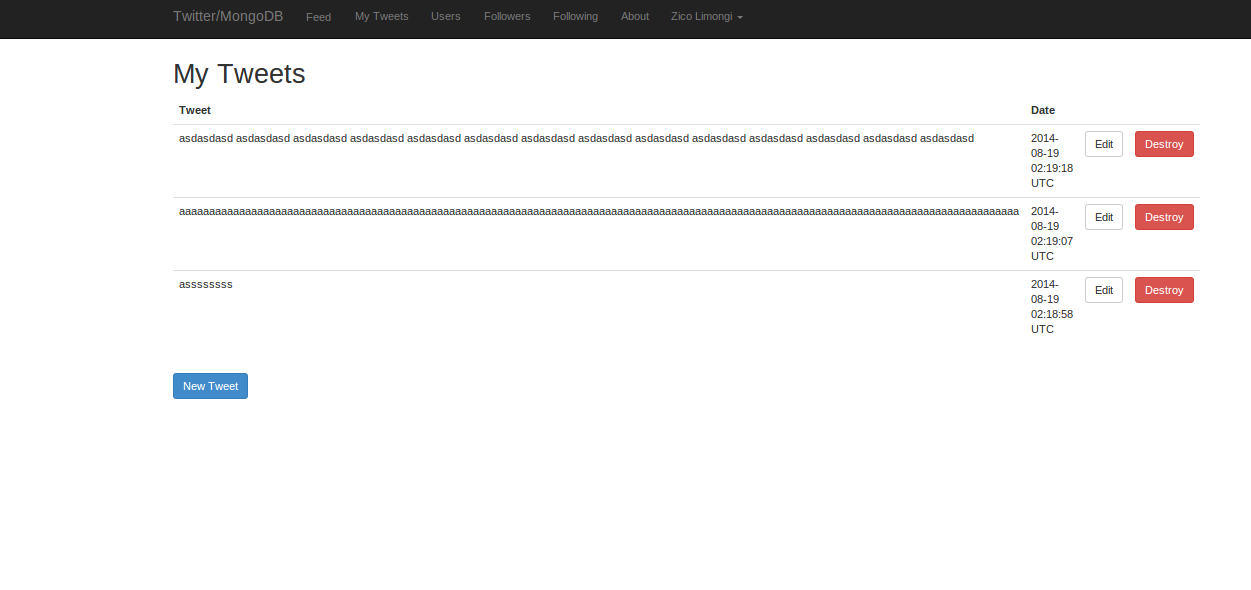
\includegraphics[width=0.8\textwidth]{./04-figuras/myTweets.png}
    \fonte{Autoria Própria}
    \label{fig:myTweets}
\end{figure}

\subsection{Caso de Uso 2 - Cadastro de \textit{tweet}}
\label{subsec:useCaseCreateTweet}

Sumário: Usuário usa o sistema para cadastrar um \textit{tweet}

Ator primário: Usuário

Ator secundário: Sistema

Precondições: O usuário deverá ser cadastrado e deve estar logado no sistema

Fluxo Principal
\begin{enumerate}
{\setlength\itemindent{25pt}
\item O usuário acessa o sistema e faz o \textit{login}, \autoref{fig:login};
\item O sistema abre a listagem dos \textit{tweets} do usuário,\autoref{fig:myTweets};
\item O usuário clica no botão \textit{New Tweet};
\item O sistema retorna com o formulário para cadastrar \textit{tweet}, \autoref{fig:createTweet};
\item O usuário escreve o \textit{tweet} no campo indicado;
\item O sistema cria um novo \textit{tweet}, registrando que o usuário é o autor do \textit{tweet}, data e hora que foi criado.
}
\end{enumerate}
\begin{figure}[H]
    \centering
    \caption{Tela de Login}
    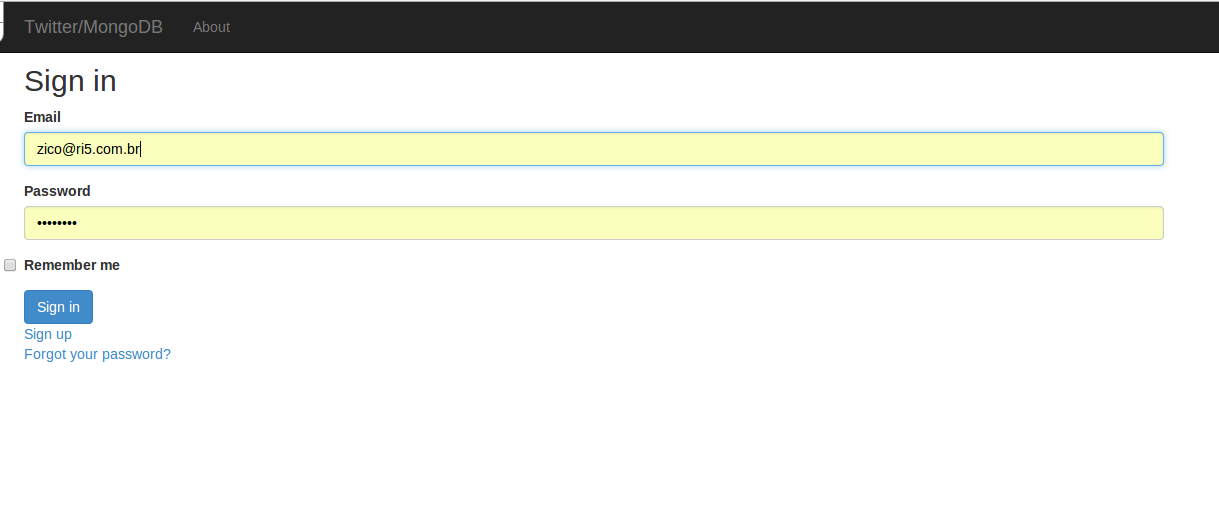
\includegraphics[width=0.8\textwidth]{./04-figuras/login.png}
    \fonte{Autoria Própria}
    \label{fig:login}
\end{figure}
\begin{figure}[H]
    \centering
    \caption{Tela Cadastro de Tweet}
    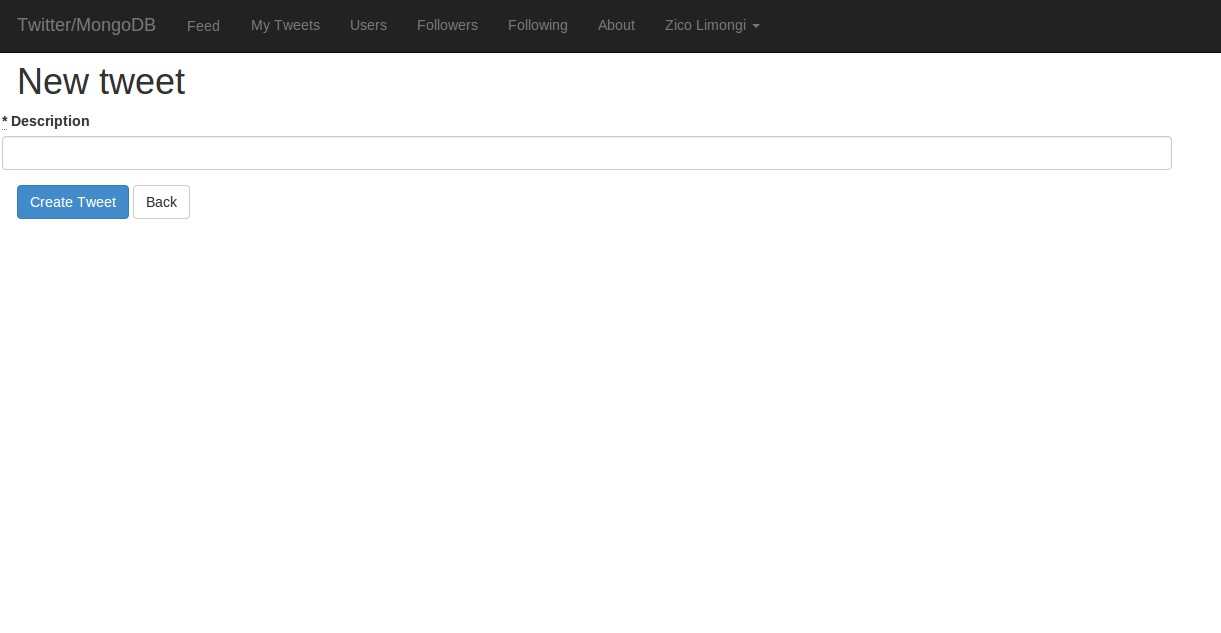
\includegraphics[width=0.8\textwidth]{./04-figuras/createTweet.png}
    \fonte{Autoria Própria}
    \label{fig:createTweet}
\end{figure}


\subsection{Caso de Uso 3 - Usuário segue outro usuário}
\label{subsec:useCaseUserFollow}

Sumário: Usuário segue outro usuário

Ator primário: Usuário

Ator secundário: Sistema

Precondições: O usuário deverá ser cadastrado e deve estar logado no sistema

Fluxo Principal
\begin{enumerate}
{\setlength\itemindent{25pt}
\item O usuário acessa o sistema e faz o \textit{login},\autoref{fig:login};
\item O sistema abre a listagem dos \textit{tweets} do usuário, \autoref{fig:myTweets};
\item O usuário clica no menu \textit{Users};
\item O sistema retorna a listagem paginada com todos os usuários cadastrados, \autoref{fig:users};
\item O usuário escolhe algum usuário que deseja seguir e clica no botão \textit{Follow};
\item O sistema armazena essa informação.
}
\end{enumerate}

\begin{figure}[H]
    \centering
    \caption{Tela de Listagem de Usuários}
    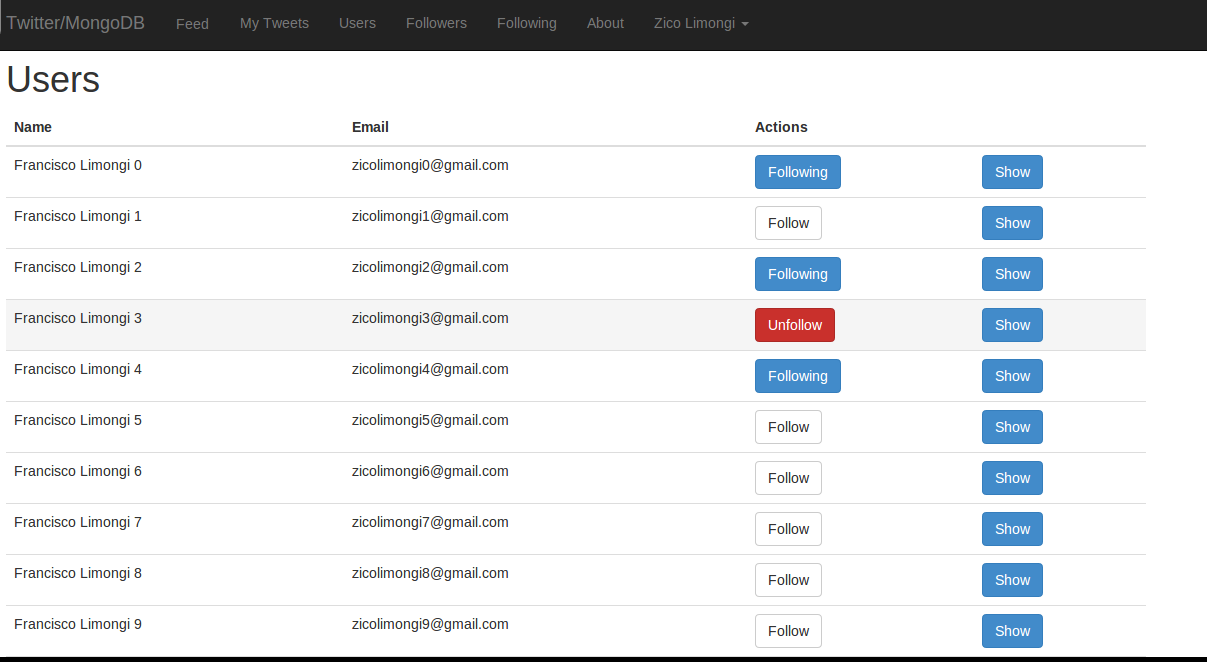
\includegraphics[width=0.8\textwidth]{./04-figuras/users.png}
    \fonte{Autoria Própria}
    \label{fig:users}
\end{figure}

\subsection{Caso de Uso 4 - Usuário para de seguir algum usuário}
\label{subsec:useCaseUserUnfollow}

Sumário: Usuário para de seguir algum usuário

Ator primário: Usuário

Ator secundário: Sistema

Precondições: O usuário deverá ser cadastrado e deve estar logado no sistema. Além disso, o usuário logado deve estar seguindo o usuário que ele deseja parar de seguir

Fluxo Principal
\begin{enumerate}
{\setlength\itemindent{25pt}
\item O usuário acessa o sistema e faz o \textit{login}, \autoref{fig:login};
\item O sistema abre a listagem dos \textit{tweets} do usuário, \autoref{fig:myTweets};
\item O usuário clica no menu \textit{Users};
\item O sistema retorna a listagem paginada com todos os usuários cadastrados, \autoref{fig:users};
\item O usuário encontra o usuário que deseja parar seguir e clica no botão \textit{Unfollow};
\item O sistema armazena essa informação.
}
\end{enumerate}

\subsection{Caso de Uso 5 - Usuário visualiza a \textit{feed}}
\label{subsec:useCaseFeed}

Sumário: Usuário visualiza os \textit{tweets} dos usuários que ele segue

Ator primário: Usuário

Ator secundário: Sistema

Precondições: O usuário deverá ser cadastrado e deve estar logado no sistema. Além disso, o usuário logado deve estar seguindo algum usuário

Fluxo Principal
\begin{enumerate}
{\setlength\itemindent{25pt}
\item O usuário acessa o sistema e faz o \textit{login}, \autoref{fig:login};
\item O sistema abre a listagem dos \textit{tweets} do usuário, \autoref{fig:myTweets};
\item O usuário clica no menu \textit{Feed};
\item O sistema retorna a listagem paginada com todos os \textit{tweets} dos usuários que o ator primário segue, \autoref{fig:feed}.
}
\end{enumerate}

\begin{figure}[H]
    \centering
    \caption{Tela de Feed}
    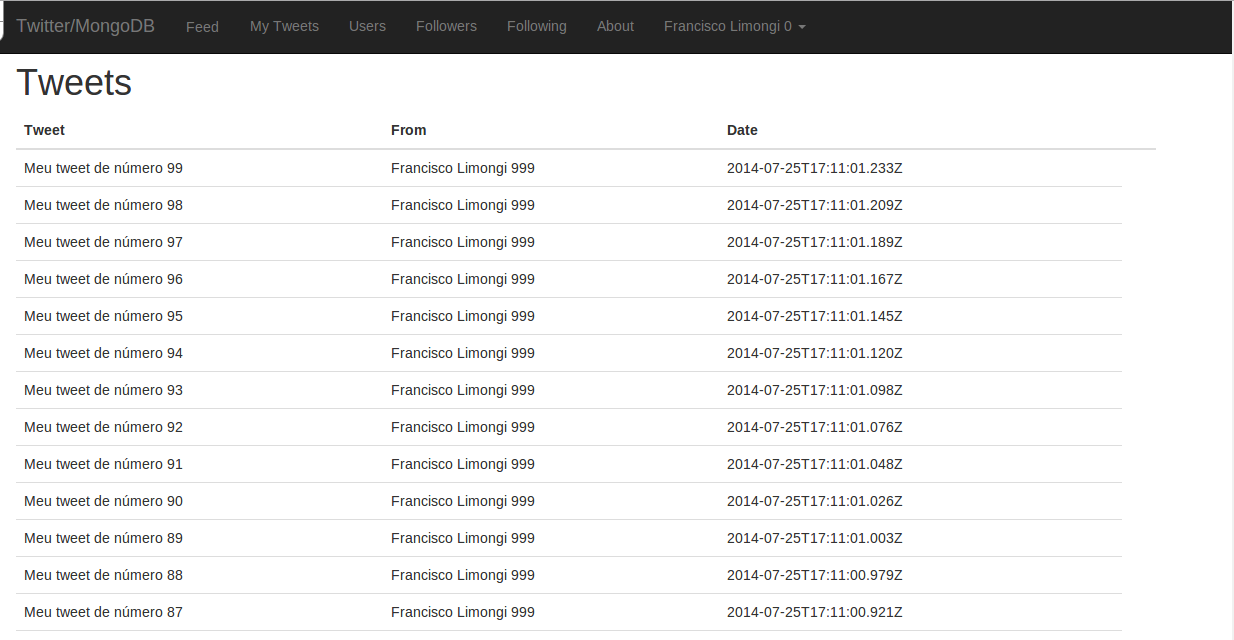
\includegraphics[width=0.8\textwidth]{./04-figuras/feed.png}
    \fonte{Autoria Própria}
    \label{fig:feed}
\end{figure}


\section{Sistema Desenvolvido}
\label{sec:applications}

Ambos os sistemas foram desenvolvidos na linguagem \textit{ruby} com o \textit{framework rails}. Esse \textit{framework} é próprio para Web e utiliza a arquitetura de \textit{software} \ac{MVC}. Além disso, é uma ferramenta de desenvolvimento ágil, que facilita o desenvolvimento Web.
Foram utilizado outras \textit{gems} \footnote{\textit{Gem} é análogo a biblioteca nas outras linguagens}, a lista utilizada em cada aplicação criada se encontra no arquivo chamado Gemfile.lock. Podemos destacar a \textit{gem} Devise \footnote{\url{https://github.com/plataformatec/devise}} e a \textit{gem} MongoId \footnote{\url{http://mongoid.org/}} como principais. A Devise faz o controle de sessão do usuário e a Mongoid deixa transparente para o desenvolvedor a comunicação com o banco de dados MongoDB. Também utilizamos a \textit{gem} bootstrap-sass para melhorar usabilidade da aplicação.

Esta seção foi dividida em duas subseções. A \autoref{subsec:monoglot} descreve os detalhes de implementação do sistema monoglota. e a \autoref{subsec:polyglot}  descreve os detalhes da implementação poliglota.

A seguir apresentamos os detalhes de implementação de cada sistema.

\subsection{Implementação com Persistência Monoglota}
\label{subsec:monoglot}

Essa implementação utiliza apenas o banco de dados MongoDB que é orientado a documento. O código da aplicação está disponível no GitHub \footnote{\url{https://github.com/zicolimongi/Twitter-Mongo}}.

Na camada de modelos temos apenas duas classes, \verb|Tweet| e \verb|User|. A classe \verb|Tweet| representa o \textit{tweet} e a classe \verb|User| representa o usuário. Ambos são armazenados como coleção no MongoDB. Cada objeto de uma dessas classes é um documento. Na \autoref{fig:diagrama_models} podemos visualizar o relacionamento entre as classes.
\begin{figure}[H]
    \centering
    \caption{Camada de modelo}
    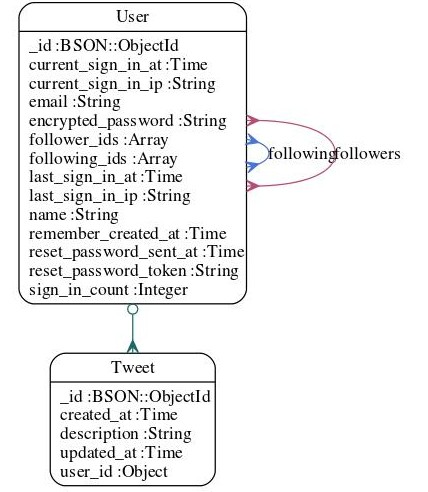
\includegraphics[width=0.5\textwidth]{./04-figuras/models_complete.jpg}
    \fonte{\cite{NoSQL}}
    \label{fig:diagrama_models}
\end{figure}
A classe \verb|Tweet| armazena identificador do próprio \textit{tweet}, data de criação, data da última atualização desse objeto, descrição do \textit{tweet} e o identificador do usuário que criou o \textit{tweet}. Não escolhemos usar agregação nessa relação, pois umas das principais perspectivas é visualizar os \verb|Tweets| de diferentes usuários. Nessa classe temos duas validações: uma de presença do campo descrição e outra que limita o tamanho desse campo em cento e quarenta caracteres.

A classe \verb|User| armazena o identificador do usuário, email, nome, uma série de campos usados para autenticação, data de criação do objeto, data da última modificação do objeto, lista de usuários seguidos e a lista de usuários seguidores. A classe \verb|User| tem três relacionamentos, um com \verb|Tweet| que já foi citado e dois autorrelacionamentos para armazenar a lista de usuários que seguem e que são seguidos. Esse autorrelacionamento no banco de dados orientado a documento funciona de uma maneira diferente do banco de dados relacional.
Enquanto no modelo relacional é necessário criar uma nova tabela, no modelo não-relacional armazenamos apenas as listas com os identificadores dos usuários, pois é permitido valores multivalorados. Logo, basta armazenar os identificadores da relação em uma lista embutida no documento do usuário. Então temos uma lista que armazena os identificadores dos usuários que são seguidos, chamada de \verb|following| e outra lista com os identificadores dos usuários que são seguidores, chamada de \verb|followers|.
Essa classe tem três validações de presença: uma para o campo nome, outra para o campo email e a terceira para o campo de senha.

Na camada de controle temos uma hierarquia de classes conforme mostra a \autoref{fig:diagrama_controllers}. \verb|ApplicationController| é a classe de controle que herda da classe do \textit{framework}. Em seguida, temos o \verb|HomeController| e \verb|Logged::BaseController| que herda  da classe \verb|ApplicationController|. \verb|HomeController| é a classe responsável por implementar o controle das páginas de \verb|about| e \verb|index|. Já o \verb|Logged::BaseController| é a classe responsável por carregar o layout do usuário logado e verificar a autenticidade do usuário.
Abaixo do \verb|Logged:BaseController| foram criadas mais duas classes: \verb|TweetsController| e \verb|UsersController| que implementam os controles de \textit{tweets} e usuários respectivamente.
\begin{figure}[H]
    \centering
    \caption{Camada de controle}
    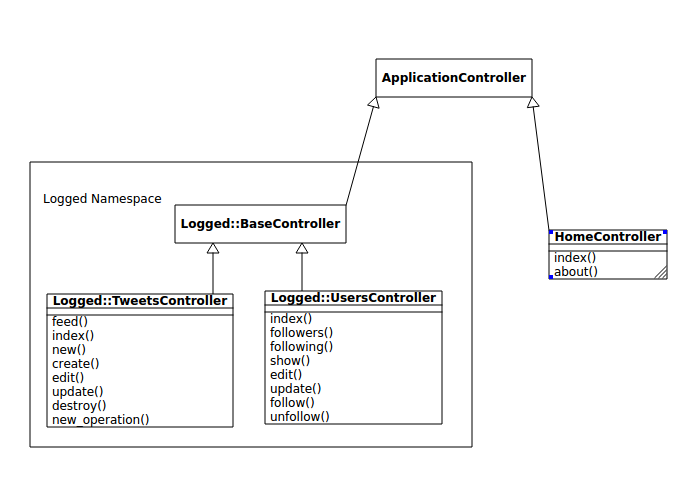
\includegraphics[width=0.8\textwidth]{./04-figuras/controllers_complete.png}
    \fonte{\cite{NoSQL}}
    \label{fig:diagrama_controllers}
\end{figure}

Toda consulta que resulte em mais de trinta registros são paginadas, isto é, colocamos um limite para que o banco não busque mais que 30 registros de uma só vez. Isso funciona manipulando duas variáveis \verb|offset| e \verb|limite|. Também devemos ressaltar que
antes de todas ações é executado uma consulta, no banco, que carrega para variável \verb|current_user| o usuário logado, caso exista. Essa busca é feita pela \textit{gem} Devise e é transparente para o desenvolvedor.

O controle de usuário implementa as ações \verb|index|, \verb|followers|, \verb|following|, \verb|show|, \verb|edit|, \verb|update|, \verb|follow| e \verb|unfollow|, todas descritas a seguir:

A ação \verb|index| lista todos os usuários com exceção do usuário logado. Na página renderizada, o usuário logado poderá seguir os usuários que ele ainda não segue, ou poderá parar de seguir os usuários que ele segue. É realizado apenas uma consulta para ler os usuários do sistema.

A ação \verb|followers| lista todos os usuários que seguem o usuário logado. Na página renderizada, o usuário logado poderá seguir os usuários que ele ainda não segue, ou poderá parar de seguir os usuários que ele já segue. É realizado apenas uma consulta no banco de dados que busca todos os usuários que o usuário logado segue.

A ação \verb|followings| lista todos os usuários que o usuário logado segue. Na página renderizada, o usuário logado poderá parar de seguir os usuários que ele segue. Da mesma maneira que a ação \verb|followers|, é realizado apenas uma consulta, porém busca os usuários que seguem o usuário logado.

A ação \verb|show| recebe um identificador como parâmetro e localiza o usuário que possui esse identificador. A página renderizada mostra o nome e email do usuário localizado e os \textit{tweets} que ele fez. Nessa página, são realizadas duas consultas, uma que busca o usuário e outra que busca os \textit{tweets} desse usuário.

A ação \verb|edit| renderiza o formulário de edição para que o usuário logado possa mudar algum campo, como nome, email ou senha. Nessa ação nenhuma consulta adicional é feita.

A ação \verb|update| recebe os parâmetros das alterações que o usuário fez no próprio perfil e registra isso no banco de dados. É realizado uma escrita no banco de dados para atualizar esses dados passados por parâmetro.

A ação \verb|follow| recebe como parâmetro o usuário que será seguido pelo usuário logado e registra esse relacionamento. Para isso é necessário uma consulta para ler qual usuário será seguido e duas escritas: uma para atualizar o usuário que está sendo seguido com o identificador do usuário seguidor e outra para atualizar o usuário seguidor com o identificador do usuário seguido.

A ação \verb|unfollow| recebe como parâmetro o usuário que deixará de ser seguido pelo usuário logado e apaga o registro desse relacionamento. Para isso é necessário uma consulta para ler o usuário que deixará de ser seguido e duas escritas no banco de dados: uma para atualizar a lista de seguidores do usuário que deixou de ser seguido outra para atualizar a lista de seguindo do usuário seguidor que deixou de seguir.

O controle de \textit{tweets} implementa as ações \verb|feed|, \verb|index|, \verb|new|, \verb|edit|, \verb|update| e \verb|destroy|, descritas a seguir:

A ação \verb|feed| é responsável por fazer a busca no banco de dados dos \textit{tweets} de todos os usuários que o usuário logado segue, ordenado-os pela data de criação de forma descendente, isto é, do \textit{tweet} mais recente para o mais antigo.

A ação de \verb|index| lista todos os \textit{tweets} do usuário logado, para isso foi necessário fazer apenas uma consulta no banco de dados que busca esses \textit{tweets}.

A ação \verb|new| renderiza o formulário de cadastro de \textit{tweet}, não é feito nenhuma consulta adicional.

A ação \verb|create| recebe como parâmetro o campo de descrição do \textit{tweet}, relaciona esse \textit{tweet} com o usuário logado e faz a escrita no desse no banco, caso seja válido.

A ação \verb|update| recebe como parâmetro o campo de descrição e o identificador do \textit{tweet} que será alterado, faz a leitura no banco de dados desse tweet com o identificador passado. Em seguida, altera o valor da descrição e faz a escrita no banco de dados.

A ação \verb|destroy| recebe como parâmetro o identificador do \textit{tweet} que será excluído, em seguida faz a leitura desse \textit{tweet} para verificar se o usuário logado é o autor do \textit{tweet} e caso seja confirmado, faz exclusão desse do banco de dados.


\subsection{Implementação com Persistência Poliglota}
\label{subsec:polyglot}

Para fazer a aplicação com persistência poliglota foi feito uma cópia da aplicação com persistência monoglota e em seguida feito as alterações necessárias para que o segundo banco de dados fosse usado. O código da aplicação está disponível no GitHub\footnote{\url{https://github.com/zicolimongi/Twitter-Mongo-Redis}}.
Na aplicação monoglota a única maneira de consultar os \textit{tweets} na \verb|feed| é buscar todos os \textit{tweets}, cujos o autores estejam na lista de \verb|followers| do usuário logado. Para isso, era necessário varrer \textit{tweet} por \textit{tweet} e verificar se o autor está na lista. Pensando nessa abordagem utilizamos a persistência poliglota para melhorar o tempo de leitura da \verb|feed| de \textit{tweets}.
Então utilizamos um segundo banco de dados, do gênero chave-valor, chamado \ac{Redis}, que armazena os cem \textit{tweets} mais recentes, cujos o autores estão na lista de \verb|followers| do usuário logado.
O \ac{Redis} irá armazenar esses cem \textit{tweets} em uma chave com o identificador do usuário concatenada com a string \verb|"_feed"| , ou seja, o usuário que tem o identificador igual a um, a chave será \verb|"1_feed"| . Todo usuário terá uma chave que armazenará os \textit{tweets} da \verb|feed|. Quando ele for acessar a página de \verb|feed|, ao invés do sistema fazer a consulta no MongoDB e varrer \textit{tweet} por \textit{tweet}, ele irá apenas consultar o \ac{Redis} com a chave e será retornado o valor com os cem \textit{tweets} mais recentes que o usuário logado segue.


Para persistir esses dados no \ac{Redis}, precisamos alterar o sistema na camada de controle e na camada de modelo. Inicialmente foi necessário instalar outra \textit{gem}, chamada redis \footnote{\url{https://github.com/antirez/redis}}, que faz a comunicação com o banco de dados chave-valor. Em seguida, implementamos três métodos na classe \verb|User|: \verb|feed_key|, \verb|remake_feed| e \verb|update_tweet_hash|, descritos a seguir:

O método \verb|feed_key| foi criado apenas para retornar a chave que será usada para armazenar no \ac{Redis}.

O método \verb|remake_feed| foi criado para refazer o valor da \verb|feed| de algum usuário quando necessário. Após fazer a implementação poliglota, utilizamos esse método para popular o \ac{Redis}.

O método \verb|update_tweet_hash| foi implementado para adicionar mais um \textit{tweet} na \verb|feed| de \textit{tweets} do usuário.

Também precisamos adicionar três métodos na classe \verb|Tweet|: o método \verb|feed_of|, \verb|to_redis_json|,\verb|update_hash|.

O método \verb|feed_of| é estático, pois irá trazer uma coleção de \textit{tweets}. Esse método recebe como parâmetro um usuário, acessa o redis com a chave desse usuário e em seguida, faz um parse do valor lido, que foi armazenado como JSON, para aplicação.

O método \verb|to_redis_json| é usado para converter o objeto \textit{tweet} no formato JSON para que possa ser armazenado no \ac{Redis}.

Por fim, o terceiro método criado é o \verb|update_hash|, privado, que é responsável por atualizar todas as chaves com o \textit{tweet} que foi criado. Esse método é executado por um \textit{callback}, chamado \verb|after_create|, com isso, toda a vez que for criado um \textit{tweet} pela aplicação o método \verb|update_hash| será rodado.

Ainda foi necessário modificar o controle de \textit{tweet}, para que a ação \verb|feed| leia os \textit{tweets} do \ac{Redis} e não do MongoDB.




           % Implementação
    %
% Documento: Resultados
%

\chapter{Análise de Resultados}

Inserir seu texto aqui...

\section{Situação atual}

Inserir seu texto aqui...

\section{Análise dos dados coletados}

Inserir seu texto aqui...

            % Resultados
    \chapter{Conclusão}
\label{chap:conclusao}

A persistência poliglota pode melhorar o desempenho da aplicação, mas o modelo deve ser bem estudado, para que haja uma melhora no sistema como um todo. Os resultados preliminares não são suficientes para provar que a persistência poliglota melhora o desempenho, pois temos que ter uma análise de espaço ocupado por esses bancos de dados, complexidade de armazená-los em um ambiente paralelo.

Este trabalho apresentado é apenas um começo do estudo de persistência poliglota. Podemos fazer diferentes análises, como a quantidade de espaço utilizado, consistência das informações e outras para afirmar qual modelo é melhor. A próxima etapa seria aprofundar os testes realizados nas duas aplicações e em seguida colocar ambas em um ambiente paralelo.


             % Conclusão

    % Elementos pós textuais
    \postextual
    %
% Documento: Referências Bibliográficas
%

\bibliography{./refbase}    % Geração automática das referências por meio do arquivo 'refbase.bib'
       % Referências
    %\include{./03-elementos-pos-textuais/glossario}        % Glossário
    %%
% Documento: Apêndices
%

\begin{apendicesenv}
\partapendices

\chapter{Nome do Apêndice}
\label{chap:apendicex}

Inserir seu texto aqui...

\chapter{Nome do Apêndice}
\label{chap:apendicey}

Inserir seu texto aqui...

\end{apendicesenv}
         % Apêndices
    %%
% Documento: Anexos
%

\begin{anexosenv}
\partanexos

\chapter{Nome do Anexo}
\label{chap:anexox}

Inserir seu texto aqui...

\chapter{Nome do Anexo}
\label{chap:anexoy}

Inserir seu texto aqui...

\end{anexosenv}            % Anexos
    \printindex                                             % Índice remissivo

\end{document}
